\chapter{Packed Pre-Constructed Publicly Verifiable Secret Sharing}
\label{cha:3}
In most of the real time distributed applications, each participant runs as a dealer once to share their 
secrets with other participants. To retrieve back the secrets, remaining participants need to open their 
shares and perform a bunch of operations, which requires a lot of communication 
amongst the participants. During the whole time of secret reconstruction one could have asked to the dealer 
itself to reveal the secret which will save a lot of time and communication. This is the main motivation 
behind the work of \textit{Pre-Constructed Publicly Verifiable Secret Sharing} (PPVSS) \cite{cryptoeprint:2025/576}, 
where the authors have given the complete description of PPVSS and an example $\Lambda_{RO}$ to improve 
the original e-voting protocol proposed by Schoenmakers \cite{5581ccd9530540479539d21d1d39ae96}.\par

In this chapter we will introduce Packed Pre-Constructed Publicly Verifiable Secret Sharing (PPPVSS or 3PVSS) which merely 
is an extension to the notion of PPVSS. As Packed Shamir secret sharing \ref{sec:packed-shamir} allows a 
dealer to share multiple secrets encoded in a single polynomial, we want to extend PPVSS to Packed 
Pre-Constructed Publicly Verifiable Secret Sharing where 
multiple secrets are encoded in a single polynomial. We remark that 
the definition of PPVSS naturally extends to 3PVSS where a commitment to the secret is replaced 
by a vector of commitments of the secrets or a single commitment that represents all secrets. In the latter case 
where a single commitment is used, we will detail the assumptions due to which our protocols 
can remain secure. In the 
subsequent sections we will provide our two constructions for 3PVSS based on packed secret sharing 
scheme \ref{sec:packed-shamir} along with the security guarantees these schemes can achieve.\par

% \section{Definitions}
% \label{sec:3PVSS-definitions}

% The following definition directly follows the definition of PPVSS in \cite{cryptoeprint:2025/576}.

% \begin{definition}[Packed Pre-Constructed Publicly Verifiable Secret Sharing (3PVSS)]
%     A Packed PPVSS scheme should have four algorithms, namely, Initial, Share, Verify and Reconstruction whose 
%     descriptions are as follows:
%     \begin{itemize}
%         \item \textbf{Initial} $(1^\lambda)\rightarrow(\{PK_i,SK_i\}_{i=1}^n\sqcup\{h_j\text{ or }(PK_j,SK_j)\}_{j=-(\ell-1)}^0)$: 
%           When given $1^\lambda$, each party $P_i$ for $1\leq i\leq n$ registers their public key $PK_i$ in a 
%           public ledger and withholds the corresponding secret key $sk_i$. Also, all parties and the dealer $D$ 
%           agree on $\ell$ commitment keys or public keys whose secret keys are known to some target people. 
%           Note that the message space of the public-key scheme is a subgroup of $(\mathbb{G},\times)$.
%         \item \textbf{Share} $(n,t,\{f_j\}_{j=-(\ell-1)}^0,\{PK_i\}_{i=1}^n\bigsqcup\{h_j\text{ or }PK_j\}_{j=-(\ell-1)}^0)$\par
%           $\rightarrow(\{y_i\}_{i=-(\ell-1)}^n,\pi_{3PVSS})$:\par 
%           It secret shares $\{f_j\}_{j=(\ell-1)}^0$ to obtain the shares $\{f_i\}_{i=1}^n$. For $1\leq i\leq n$, uses 
%           the public key $PK_i$ to encrypt $f_i$ and obtain the encrypted share $y_i$. Now, it uses the commitment 
%           key $h_j$ ( or public key $PK_j$) to commit(/encrypt) $f_j$ to obtain $y_j$ for $-(\ell-1)\leq j\leq0$. 
%           In the next step, it uses a NIZK proof $\pi_{3PVSS}$ protocol to prove that $\{y_j\}_{j=-(\ell-1)}^0$ is a set of valid 
%           commitments(/encryptions) of $\ell$ secrets and $\{y_i\}_{i=1}^n$ has valid encryptions of the corresponding shares. Finally, it returns $(\{y_i\}_{i=-(\ell-1)}^n,\pi_{3PVSS})$.\par
%           \textit{\textbf{OR}}\par
%           $\rightarrow(\{y_i\}_{i=0}^n,\pi_{3PVSS})$:\par 
%           It secret shares $\{f_j\}_{j=(\ell-1)}^0$ to obtain the shares $\{f_i\}_{i=1}^n$. For $1\leq i\leq n$, uses 
%           the public key $PK_i$ to encrypt $f_i$ and obtain the encrypted share $y_i$. Now, it uses the commitment 
%           key $h_j$ ( or public key $PK_j$) to commit(/encrypt) $f_j$ for $-(\ell-1)\leq j\leq0$ and performs the 
%           group operation $\times$ to multiply all the commitments(/encryptions) to obtain $y_0$. 
%           In the next step, it uses a NIZK proof $\pi_{3PVSS}$ protocol to prove that $y_0$ is a valid well-formed commitment of $\ell$ 
%           secrets and $\{y_i\}_{i=1}^n$ has valid encryptions of the corresponding shares. Finally, it returns $(\{y_i\}_{i=0}^n,\pi_{3PVSS})$.
%         \item \textbf{Verify} $(n,t,\ell,\{y_i\}_{i=-(\ell-1)}^n,\pi_{3PVSS})\rightarrow$ \textbf{true/false}: 
%           This algorithm(which can be performed by anyone) checks if the NIZK proof $\pi_{3PVSS}$ is valid for 
%           $\{y_{-(\ell-1)},\dots,y_0,\dots,y_n\}$ and then returns true, otherwise false.\par
%           \textit{\textbf{OR}}\par
%           \textbf{Verify} $(n,t,\ell,\{y_i\}_{i=0}^n,\pi_{3PVSS})\rightarrow$ \textbf{true/false}: 
%           This algorithm(which can be performed by anyone) checks if the NIZK proof $\pi_{3PVSS}$ is valid for 
%           $\{y_0,y_1,\dots,y_n\}$ and then returns true, otherwise false.
%         \item \textbf{Reconstruct}: There are two approaches based on cooperation of the dealer $D$ and are as follows:
%           \begin{itemize}
%             \item \textbf{(Optimistic)} $Reconstruction^{opt}[\{h_j,f_j,r_j,y_j\}_{j=-(\ell-1)}^0\text{ or }\{PK_j,SK_j,y_j\}_{j=-(\ell-1)}^0]$\par$\rightarrow(\{f_j\}_{j=-(\ell-1)}^0\text{ or }false)$:
%               \begin{itemize}
%                 \item Given the input a verifier checks if $\{y_j\}_{j=-(\ell01)}^0$ is a valid set of commitments of the $\ell$ secrets. 
%                  If so, it returns $\{f_j\}_{j=-(\ell-1)}^0$; otherwise it returns $false$.
%                 \item Given the public keys with their corresponding secret keys,\par $\{(PK_j,SK_j)\}_{j=-(\ell-1)}^0$ 
%                  a verifier checks if $\{y_j\}_{j=-(\ell-1)}^0$ is a valid set of encryptions of the $\ell$ secrets. 
%                  If so, it returns $\{f_j\}_{j=-(\ell-1)}^0$; otherwise it returns $false$.
%               \end{itemize}\par
%               \textit{\textbf{OR}}\par
%               \textbf{(Optimistic)} $Reconstruction^{opt}[(\{h_j,f_j,r_j\}_{j=-(\ell-1)}^0,y_0)\text{ or }(\{PK_j,SK_j\}_{j=-(\ell-1)}^0,y_0)]$\par$\rightarrow(\{f_j\}_{j=-(\ell-1)}^0\text{ or }false)$:
%               \begin{itemize}
%                 \item Given the commitment keys $\{h_j\}_{j=-(\ell-1)}^0$, $y_0$ and $\ell$ secrets, $\{f_j,r_j\}_{j=-(\ell-1)}^0$, 
%                  a verifier checks if $y_0$ is a valid well-formed commitment of the $\ell$ secrets constructed by taking the product of commitment of $\ell$ secrets. If so, it returns 
%                  $\{f_j\}_{j=-(\ell-1)}^0$; otherwise it returns $false$.
%                 \item Given the public keys with their corresponding secret keys,\par $\{(PK_j,SK_j)\}_{j=-(\ell-1)}^0$ 
%                  a verifier checks if $y_0$ is a valid well-formed commitment of the $\ell$ secrets constructed by taking the product of encryptions of $\ell$ secrets. 
%                  If so, it returns $\{f_j\}_{j=-(\ell-1)}^0$; otherwise it returns $false$.
%               \end{itemize}
%             \item \textbf{(Pessimistic)} $Reconstruction^{pes}[\{y_i,SK_i\}_{i\in\mathcal{Q},|\mathcal{Q}|=t+\ell}]\rightarrow(\{f_j\}_{j=-(\ell-1)}^0\text{ or }false))$: 
%               Given any $t+\ell$ encrypted shares along with corresponding secret keys, it outputs the secrets 
%               $\{f_j\}_{j=-(\ell-1)^0}$ or $false$. This can be done in two phases as follows: 
%                 \begin{itemize}
%                   \item \textbf{Decryption of the shares}, each party $P_i\in\mathcal{Q}$ decrypts $y_i$ to obtain 
%                     $f_i$ using its secret key $SK_i$. Then it generates a NIZK proof $\pi_i^{Dec}$ which proves that 
%                     $f_i$ is the correct decryption of $y_i$. Now, $P_i$ publishes $(f_i,\pi_i^{Dec})$.
%                   \item \textbf{Share pooling}, a verifier $V$ (not necessarily from the shareholders) checks if proof 
%                    $\pi_i^{Dec}$ is correct for each $P_i\in\mathcal{Q}$. If any check fails, then $V$ returns $false$; 
%                    otherwise $V$ applies a reconstruction procedure to the set of valid shares, $\{f_i\}_{i\in\mathcal{Q},|\mathcal{Q}|=t+\ell}$, 
%                    and returns $\{f_j\}_{j=-(\ell-1)}^0$.
%                 \end{itemize}
%           \end{itemize}
%     \end{itemize}
% \end{definition}

% We need following security guarantees (inspired from PPVSS \cite{cryptoeprint:2025/576}) for a 3PVSS to be 
% called secure:

% \begin{itemize}
%   \item \textbf{Correctness}: If the dealer and parties follow the protocol, then the \textit{\textbf{Verify}} 
%     algorithm returns \textit{\textbf{true}} and the \textit{\textbf{Reconstruct}} algorithm returns $\{f_j\}_{j=-(\ell-1)}^0$ 
%     irrespective of which approach. For any integer $n\geq t+\ell$ with $t>0$, a 3PVSS is said 
%     to be correct for\par 
%     $\left(\{PK_i,SK_i\}_{i=1}^n\sqcup\{h_j\text{ or }(PK_j,SK_j)\}_{j=-(\ell-1)}^0\right)\leftarrow$\textbf{Initial} $(1^\lambda)$ when 
%     it satisfies either of the two formal definitions based on the output of the \textit{Share} algorithm 
%     and they are as follows: 
%     \begin{itemize}
%       \item When \textit{Share} algorithm outputs $\ell$ commitments(/encryptions) of the secrets, then
%         \begin{align*}
%           Pr\begin{bmatrix}
%             (\{y_i\}_{i=-(\ell-1)}^n,\pi_{3PVSS})&\leftarrow \textit{\textbf{Share}} \big(n,t,\{f_j\}_{j=-(\ell-1)}^0,\{PK_i\}_{i=1}^n\bigsqcup\\
%             &\{h_j\text{ or }PK_j\}_{j=-(l-1)}^0\big):\\
%             \textit{\textbf{true}}&\leftarrow \textit{\textbf{Verify}} (n,t,\ell,\{y_i\}_{i=-(\ell-1)}^n,\pi_{3PVSS})
%           \end{bmatrix} = 1,
%         \end{align*}
    
%         \begin{align*}
%           Pr\begin{bmatrix}
%             (\{y_i\}_{i=-(\ell-1)}^n,\pi_{3PVSS})&\leftarrow \textit{\textbf{Share}} \big(n,t,\{f_j\}_{j=-(\ell-1)}^0,\{PK_i\}_{i=1}^n\bigsqcup\\
%             &\{h_j\text{ or }PK_j\}_{j=-(l-1)}^0\big),\\
%             \{f_j^{'}\}_{j=-(\ell-1)}^0&\leftarrow Reconstruction^{opt}[\{h_j,f_j,r_j,y_j\}_{j=-(\ell-1)}^0\\
%             &\textit{ or }\{PK_j,SK_j,y_j\}_{j=-(\ell-1)}^0]\bigvee\\
%             \{f_j^{'}\}_{j=-(\ell-1)}^0&\leftarrow Reconstruction^{pes}[\{y_i,SK_i\}_{i\in\mathcal{Q},|\mathcal{Q}|=t+\ell}]:\\
%             &f_j^{'}=f_j,-(\ell-1)\leq j\leq 0
%           \end{bmatrix} = 1,
%         \end{align*}
%       \item When \textit{Share} algorithm outputs a single commitment corresponding to the $\ell$ secrets, then
%         \begin{align*}
%           Pr\begin{bmatrix}
%             (\{y_i\}_{i=0}^n,\pi_{3PVSS})&\leftarrow \textit{\textbf{Share}} \big(n,t,\{f_j\}_{j=-(\ell-1)}^0,\{PK_i\}_{i=1}^n\bigsqcup\\
%             &\{h_j\text{ or }PK_j\}_{j=-(l-1)}^0\big):\\
%             \textit{\textbf{true}}&\leftarrow \textit{\textbf{Verify}} (n,t,\ell,\{y_i\}_{i=0}^n,\pi_{3PVSS})
%           \end{bmatrix} = 1,
%         \end{align*}
    
%         \begin{align*}
%           Pr\begin{bmatrix}
%             (\{y_i\}_{i=0}^n,\pi_{3PVSS})&\leftarrow \textit{\textbf{Share}} \big(n,t,\{f_j\}_{j=-(\ell-1)}^0,\{PK_i\}_{i=1}^n\bigsqcup\\
%             &\{h_j\text{ or }PK_j\}_{j=-(l-1)}^0\big),\\
%             \{f_j^{'}\}_{j=-(\ell-1)}^0&\leftarrow Reconstruction^{opt}[(\{h_j,f_j,r_j\}_{j=-(\ell-1)}^0,y_0)\\
%             &\textit{ or }(\{PK_j,SK_j\}_{j=-(\ell-1)}^0,y_0)]\bigvee\\
%             \{f_j^{'}\}_{j=-(\ell-1)}^0&\leftarrow Reconstruction^{pes}[\{y_i,SK_i\}_{i\in\mathcal{Q},|\mathcal{Q}|=t+\ell}]:\\
%             &f_j^{'}=f_j,-(\ell-1)\leq j\leq 0
%           \end{bmatrix} = 1,
%         \end{align*}
%     \end{itemize}
%   \item \textbf{Verifiability}: If \textit{\textbf{Verify}} returns \textit{\textbf{true}}, then 
%     \textit{\textbf{(Optimistic)}} $Reconstruct^{opt}$ and/or \textit{\textbf{(Pessimistic)}} $Reconstruct^{pes}$ 
%     output being $\{f_j\}_{j=-(\ell-1)}^0$ are the actual secrets of whom the shares are encrypted. Moreover, 
%     $\{y_i\}_{i=1}^n$ are valid encryptions of the shares of actual secret shares of those $\ell$ secrets with 
%     high probability and either of the following two statements is true.
%     \begin{itemize}
%       \item $\{y_j\}_{j=-(\ell-1)}^0$ are valid commitments(/encryptions) of those $\ell$ secrets with high 
%         probability. More formally, given $\lambda$, for any integers 
%         $n\geq 2t+\ell$, $\ell\geq 1$ and $t>0$, a 3PVSS is said to be verifiable if for any 
%         $\mathcal{PPT}$ adversary $\mathcal{A}$, we have:
%         \begin{align*}
%           Pr\begin{bmatrix}
%             \big(\{PK_i,SK_i\}_{i=1}^n\sqcup&\{h_j\text{ or }(PK_j,SK_j)\}_{j=-(\ell-1)}^0\big)\leftarrow\textbf{ Initial } (1^\lambda),\\
%             (\{y_i\}_{i=-(\ell-1)}^n,\pi_{3PVSS})&\leftarrow \mathcal{A} \big(n,t,\{f_j\}_{j=-(\ell-1)}^0,\{PK_i\}_{i=1}^n\bigsqcup\\
%             &\{h_j\text{ or }PK_j\}_{j=-(l-1)}^0\big),\\
%             \{f_j^{'}\}_{j=-(\ell-1)}^0&\leftarrow Reconstruction^{opt}[\{h_j,f_j,r_j,y_j\}_{j=-(\ell-1)}^0\\
%             &\textit{ or }\{PK_j,SK_j,y_j\}_{j=-(\ell-1)}^0]\bigvee\\
%             \{f_j^{'}\}_{j=-(\ell-1)}^0&\leftarrow Reconstruction^{pes}[\{y_i,SK_i\}_{i\in\mathcal{Q},|\mathcal{Q}|=t+\ell}]:\\
%             \textit{\textbf{true}}&\leftarrow \textit{\textbf{Verify}} (n,t,\ell,\{y_i\}_{i=-(\ell-1)}^n,\pi_{3PVSS})\\
%             \bigwedge f_j^{'}\neq f_j&\text{ for some }-(\ell-1)\leq j\leq 0
%           \end{bmatrix} \leq negl(\lambda),
%         \end{align*}
%         where $\mathcal{Q}$ is the set of honest parties.
%       \item $y_0$ is a valid well-formed commitment of the same $\ell$ secrets constructed by taking a 
%         product of valid commitments (/ciphers) of $\ell$ secrets under 
%         $\{h_j\textit{ or }PK_j\}_{j=-(\ell-1)}^0$. More formally, given $\lambda$, for any integers 
%         $n\geq 2t+\ell$, $\ell\geq 1$ and $t>0$, a 3PVSS is said to be verifiable if for any 
%         $\mathcal{PPT}$ adversary $\mathcal{A}$, we have:
%         \begin{align*}
%           Pr\begin{bmatrix}
%             \big(\{PK_i,SK_i\}_{i=1}^n\sqcup&\{h_j\text{ or }(PK_j,SK_j)\}_{j=-(\ell-1)}^0\big)\leftarrow\textbf{ Initial } (1^\lambda),\\
%             (\{y_i\}_{i=0}^n,\pi_{3PVSS})&\leftarrow \mathcal{A} \big(n,t,\{f_j\}_{j=-(\ell-1)}^0,\{PK_i\}_{i=1}^n\bigsqcup\\
%             &\{h_j\text{ or }PK_j\}_{j=-(l-1)}^0\big),\\
%             \{f_j^{'}\}_{j=-(\ell-1)}^0&\leftarrow Reconstruction^{opt}[(\{h_j,f_j,r_j\}_{j=-(\ell-1)}^0,y_0)\\
%             &\textit{ or }(\{PK_j,SK_j\}_{j=-(\ell-1)}^0,y_0)]\bigvee\\
%             \{f_j^{'}\}_{j=-(\ell-1)}^0&\leftarrow Reconstruction^{pes}[\{y_i,SK_i\}_{i\in\mathcal{Q},|\mathcal{Q}|=t+\ell}]:\\
%             \textit{\textbf{true}}&\leftarrow \textit{\textbf{Verify}} (n,t,\ell,\{y_i\}_{i=0}^n,\pi_{3PVSS})\\
%             \bigwedge f_j^{'}\neq f_j&\text{ for some }-(\ell-1)\leq j\leq 0
%           \end{bmatrix} \leq negl(\lambda),
%         \end{align*}
%         where $\mathcal{Q}$ is the set of honest parties.
%     \end{itemize}
%   \item \textbf{IND1-Secrecy (Indistinguishability of Secrets)}: Before reconstruction phase, any amount of public 
%     information along with secret keys of at most $t$ parties excluding $\{SK_j\}_{j=-(\ell-1)}^0$ will give 
%     absolutely no information about the secrets $\{f_j\}_{j=-(\ell-1)}^0$. More formally, for integers $n>1$ and 
%     $t+\ell\leq n$, the 3PVSS is said to satisfy \textit{IND1-Secrecy} if for any $\mathcal{PPT}$ adversary $\mathcal{A}$ 
%     corrupting at most $t$ parties, excluding the owners of $\{SK_j\}_{j=-(\ell-1)}^0$, has negligible 
%     advantage in the following game \cite{cryptoeprint:2025/576} played against a challenger.
%     \begin{itemize}
%       \item The challenger runs \textit{\textbf{Initial}} $(1^\lambda)$ of 3PVSS to obtain 
%         $\{PK_i,SK_i\}_{i=1}^n\sqcup\{h_j\text{ or }(PK_j,SK_j)\}_{j=-(\ell-1)}^0$ and sends all public 
%         information along with secret information of all corrupted parties to $\mathcal{A}$.
%       \item The challenger chooses two set of secrets, $s_0=\{f_j\}_{j=-(\ell-1)}^0$ and 
%         $s_1=\{f_j^{'}\}_{j=-(\ell-1)}^0$ at random in the space of secrets. Furthermore, it chooses $b\in\{0,1\}$ 
%         uniformly at random and runs \par 
%         \textit{\textbf{Share}} $(n,t,s_0,\{PK_i\}_{i=1}^n\bigsqcup\{h_j\text{ or }PK_j\}_{j=-(\ell-1)}^0)$ 
%         algorithm of the 3PVSS scheme and obtains $(\{y_i\}_{i=0}^n,\pi_{3PVSS})$ or 
%         $(\{y_i\}_{i=-(\ell-1)}^n,\pi_{3PVSS})$. Finally, it sends all public information generated in 
%         \textit{Share} phase together with $s_b$.
%       \item $\mathcal{A}$ guesses a bit $b'\in\{0,1\}$.
%     \end{itemize}
%     The advantage of $\mathcal{A}$ is defined to be $|Pr[b'=b]-\frac{1}{2}|$.
% \end{itemize}

% It can be seen that 3PVSS is a natural extension of PPVSS, where we secret share possibly \textit{more than one} 
% secret in contrast to \textit{only one} secret in PPVSS. But one has to be very careful in the case where they 
% obtain the commitment of the secrets which is obtained via multiplication of encryptions (/commitments) of 
% actual secrets. More precisely, $y_0$ should be well formed, i.e., a dealer should not be able to cheat to 
% obtain $y_0$ by taking multiplications of random group elements, it precisely has to be multiplication of 
% encryptions (/commitments) of the actual secrets.\par 

A general construction of Shamir based PPVSS is given in \cite{cryptoeprint:2025/576}, and we extend this idea 
to give two Packed Shamir based 3PVSS outlined in figures \ref{fig:version-packed-shamir-PPPVSS} and \ref{fig:packed-shamir-PPPVSS}. 
Subsequently, we will give two practical 3PVSS schemes. 
% Before giving out the details of the 
% second 3PVSS scheme, we will first introduce a new relation, its correspondence with a problem and finally 
% a NIZK AoK protocol for a statement in the language of that relation. The reason we had to 
% introduce this new relation is because we needed it to construct our second 3PVSS scheme. 

\begin{figure}[ht]
    \centering
    \resizebox{\textwidth}{!}{ % Further reduced the scaling factor to fit the content
    \begin{tcolorbox}[title=\textbf{a PPPVSS based on Packed Shamir secret sharing \ref{sec:packed-shamir}}, width=1.2\textwidth, colframe=blue!75!black, colback=blue!10, sharp corners]
        
        \textbf{Initialization:}
            All parties $\{P_i\}_{i=1}^n$ and dealer $D$ agree on the prime field $\mathbb{Z}_q$. Also, each party 
            $P_i$ registers their public key $PK_i$ in the public ledger and all agree on a set of commitment 
            keys or public keys, $\{h_j\text{ or }PK_j\}_{j=-(\ell-1)}^0$, whose secret keys are known to target entities with 
            the cipher text space being a group $(\mathcal{G},\times)$. More importantly, all entities agree 
            on two NIZK proof protocols, one for the dealer during sharing phase $\pi_{PPPVSS}^{share}$ and the 
            other for Pessimistic reconstruction phase $\pi_{PPPVSS}^{pes}$.

        \vspace{0.5em}
        \textbf{Share:}
        \begin{itemize}
            \item Dealer $D$ samples a $t+\ell$-degree polynomial $f\in\mathbb{Z}_q[X]$ uniformly at random and 
              sets $\{f(j)=f_j\}_{j=-(\ell-1)}^0$ as the set of all secrets.
            \item For each $1\leq i\leq n$, $D$ computes $f(i)=f_i$ and and encrypts it with $PK_i$ to obtain 
              $y_i=Enc(PK_i,f_i)$. $D$ also encrypts(/commits) to the secrets $\{f_j\}_{j=-(\ell-1)}^0$ using the encryption(/commitment) 
              keys $\{h_j\text{ or }PK_j\}_{j=-(\ell-1)}^0$ to obtain $\{y_j\}_{j=-(\ell-1)}^0$. 
            \item $D$ uses the agreed upon proof system $\pi_{PPPVSS}^{share}$ to prove that they have encrypted the shares and 
              commitments(/encryptions) of $\ell$ secrets corresponding to the correct polynomial that evaluates 
              to $\ell$ secrets.
            \item $D$ broadcasts $\{y_{-(\ell-1)},\dots,y_0,\dots,y_n,\pi_{PPPVSS}^{share}\}$.
        \end{itemize}
        
        \vspace{0.5em}
        \textbf{Verification:}
            Given public keys $\{PK_i\}_{i=1}^n$ and commitment(/public) keys $\{h_j,PK_j\}_{j=-(\ell-1)}^0$, 
            any entity can check $\pi_{PPPVSS}^{share}$ to verify the correctness of the encrypted shares $\{y_i\}_{i=1}^n$ and 
            $\{y_j\}_{j=-(\ell-1)}^0$ being the commitments(/encryptions) of the $\ell$ secrets, and outputs 
            \textbf{true} or \textbf{false} accordingly.

        \vspace{0.5em}
        \textbf{Reconstruction:}
            Similar to \cite{cryptoeprint:2025/576}, there are two approaches to reconstruct the secrets 
            $\{f_j\}_{j=-(\ell-1)}^0$ based on the cooperation of the dealer $D$ which are as follows:
            \begin{itemize}
                \item \textbf{Optimistic Reconstruction:} $D$ publishes $\{f_j\}_{j=-(\ell-1)}^0$, then any verifier (not necessarily shareholders) 
                when given $\{y_j,h_j\text{ or }PK_j\}_{j=-(\ell-1)}^0$ can check if each $y_j$ is a valid commitment(/encryption) 
                of the secret $f_j$ and returns \textbf{false} if the check fails; otherwise returns 
                $\{f_j\}_{j=-(\ell-1)}^0$.
                \item \textbf{Pessimistic Reconstruction:} If $D$ refuses to reveal $\{f_j\}_{j=-(\ell-1)}^0$, then any set 
                $\mathcal{Q}$ consisting at least $t+\ell$ shareholders will do the following:
                \begin{itemize}
                    \item Each party $P_i\in\mathcal{Q}$ decrypts their share $y_i$ using their private key $SK_i$ 
                      corresponding to $PK_i$ to obtain $f_i$ and then they publish $f_i$ 
                      along with proof $\pi_{PPPVSS}^{pes}$ which proves that the $f_i$ is the correct 
                      decryption of $y_i$.
                    \item If $\mathcal{Q}$ consists at least $t+\ell$ honest parties, they can use the 
                    lagrange interpolation to compute the secrets $\{f_j\}_{j=-(\ell-1)}^0$ as follows:
                    \begin{align*}
                        f_j &= \sum_{i\in \mathcal{Q}} f_i \left[\prod_{k\in \mathcal{Q}, k\neq i}\frac{-k-j}{i-j}\right] &&, j\in\{-(\ell-1),\dots,0\} \\
                    \end{align*}
                    where $\lambda_i=\prod_{k\neq i}\frac{k}{k-i}$ are lagrange coefficients.
                \end{itemize}
            \end{itemize}
    \end{tcolorbox}
    }
    \caption[PPPVSS Scheme]{a PPPVSS based on Packed Shamir secret sharing}
    \label{fig:version-packed-shamir-PPPVSS}
\end{figure}
\begin{figure}[ht]
    \centering
    \resizebox{\textwidth}{!}{ % Further reduced the scaling factor to fit the content
    \begin{tcolorbox}[title=\textbf{PPPVSS based on Packed Shamir secret sharing \ref{sec:packed-shamir}}, width=1.2\textwidth, colframe=blue!75!black, colback=blue!10, sharp corners]
        
        \textbf{Initialization:}
            All parties $\{P_i\}_{i=1}^n$ and dealer $D$ agree on the prime field $\mathbb{Z}_q$. Also, each party 
            $P_i$ registers their public key $PK_i$ in the public ledger and all agree on a set of commitment 
            keys or public keys, $\{h_j\text{ or }PK_j\}_{j=-(\ell-1)}^0$, whose secret keys are known to target entities with 
            the cipher text space being a group $(\mathcal{G},\times)$. More importantly, all entities agree 
            on two NIZK proof protocols, one for the dealer during sharing phase $\pi_{PPPVSS}^{share}$ and the 
            other for Pessimistic reconstruction phase $\pi_{PPPVSS}^{pes}$.

        \vspace{0.5em}
        \textbf{Share:}
        \begin{itemize}
            \item Dealer $D$ samples a $t+\ell$-degree polynomial $f\in\mathbb{Z}_q[X]$ uniformly at random and 
              sets $\{f(j)=f_j\}_{j=-(\ell-1)}^0$ as the set of all secrets.
            \item For each $1\leq i\leq n$, $D$ computes $f(i)=f_i$ and and encrypts it with $PK_i$ to obtain 
              $y_i=Enc(PK_i,f_i)$. $D$ also encrypts(/commits) to the secrets $\{f_j\}_{j=-(\ell-1)}^0$ using the encryption(/commitment) 
              keys $\{h_j\text{ or }PK_j\}$ and multiplies them together to obtain $y_0$. 
            \item $D$ uses the agreed upon proof system $\pi_{PPPVSS}^{share}$ to prove that they have encrypted the shares and 
              committed to the $\ell$ secrets corresponding to the correct polynomial that evaluates to $\ell$ secrets.
            \item $D$ broadcasts $\{y_0,\dots,y_n,\pi_{PPPVSS}^{share}\}$.
        \end{itemize}
        
        \vspace{0.5em}
        \textbf{Verification:}
            Given public keys $\{PK_i\}_{i=1}^n$ and commitment(/public) keys $\{h_j,PK_j\}_{j=-(\ell-1)}^0$, 
            any entity can check $\pi_{PPPVSS}^{share}$ to verify the correctness of the encrypted shares $\{y_i\}_{i=1}^n$ and 
            $y_0$ being the commitment of the $\ell$ secrets, and outputs \textbf{true} or \textbf{false} accordingly.

        \vspace{0.5em}
        \textbf{Reconstruction:}
            Similar to \cite{cryptoeprint:2025/576}, there are two approaches to reconstruct the secrets 
            $\{f_j\}_{j=-(\ell-1)}^0$ based on the cooperation of the dealer $D$ which are as follows:
            \begin{itemize}
                \item \textbf{Optimistic Reconstruction:} $D$ publishes $\{f_j\}_{j=-(\ell-1)}^0$, then any verifier (not necessarily shareholders) 
                when given $\{h_j\text{ or }PK_j\}_{j=-(\ell-1)}^0,y_0$ can check if $y_0$ is the valid product of the commitment(/encryptions) 
                of the secrets $\{f_j\}_{j=-(\ell-1)}^0$ and returns \textbf{false} if the check fails; otherwise returns 
                $\{f_j\}_{j=-(\ell-1)}^0$.
                \item \textbf{Pessimistic Reconstruction:} If $D$ refuses to reveal $\{f_j\}_{j=-(\ell-1)}^0$, then any set 
                $\mathcal{Q}$ consisting at least $t+\ell$ shareholders will do the following:
                \begin{itemize}
                    \item Each party $P_i\in\mathcal{Q}$ decrypts their share $y_i$ using their private key $SK_i$ 
                      corresponding to $PK_i$ to obtain $f_i$ and then they publish $f_i$ 
                      along with proof $\pi_{PPPVSS}^{pes}$ which proves that the $f_i$ is the correct 
                      decryption of $y_i$.
                    \item If $\mathcal{Q}$ consists at least $t+\ell$ honest parties, they can use the 
                    lagrange interpolation to compute the secrets $\{f_j\}_{j=-(\ell-1)}^0$ as follows:
                    \begin{align*}
                        f_j &= \sum_{i\in \mathcal{Q}} f_i \left[\prod_{k\in \mathcal{Q}, k\neq i}\frac{-k-j}{i-j}\right] &&, j\in\{-(\ell-1),\dots,0\} \\
                    \end{align*}
                    where $\lambda_i=\prod_{k\neq i}\frac{k}{k-i}$ are lagrange coefficients.
                \end{itemize}
            \end{itemize}
    \end{tcolorbox}
    }
    \caption[PPPVSS Scheme]{PPPVSS based on Packed Shamir secret sharing, version 2}
    \label{fig:packed-shamir-PPPVSS}
\end{figure}

% \begin{figure}[ht]
    \centering
    \begin{tcolorbox}[title=$\pi_{PDL}^{mod}$, width=0.9\textwidth, colframe=blue!75!black, colback=blue!10, sharp corners]
        Let $(g,x_{-(\ell-1)},\dots,x_n,F_0,\dots,F_n)\in L_{g_{-(\ell-1)},\dots,g_n}^{mod-PDL}$ with its corresponding witness being $f\in\mathbb{Z}_q[X]_{\leq t+\ell-1}$ 
        where $L_{g_{-(\ell-1)},\dots,g_n}^{mod-PDL}$ is the CRS dependent language defined by 
        the relation $R_{mod-PDL}$ and $\mathcal{H}$ be a random oracle (RO).
        
        \vspace{0.5em}
        \textbf{Prover}
        \begin{itemize}
            \item Samples $r\in_{R}\mathbb{Z}_q[X]_{t+\ell-1}$ uniformly at random and sets 
                $\Gamma=\prod_{i=-(\ell-1)}^{n}g_i^{r(x_i)}$.
            \item Sets $d\leftarrow \mathcal{H}(F_0, \dots, F_n, \Gamma)$, where $\mathcal{H}$ is 
                an agreed upon Random Oracle (RO).
            \item Sets $z(X)\equiv r(X)+df(X) \pmod{q}$ and returns the proof(/transcript) $\pi:= (d,z(X))$.
        \end{itemize}
        
        \vspace{0.5em}
        \textbf{Verifier}
        \begin{itemize}
            \item First checks if $z$ is at most a $t+\ell-1$ degree polynomial in $\mathbb{Z}_q[X]$. If so, they proceed with the next step.
            \item Checks if $d\leftarrow \mathcal{H}(F_0, \dots, F_n,\frac{\prod_{i=-(\ell-1)}^{n}g_i^{z(x_i)}}{[\prod_{i=0}^{n}F_i]^d})$. 
            \item If first two steps are correct then they output \textbf{true}, otherwise \textbf{false}.
        \end{itemize}
    \end{tcolorbox}
    \caption{A NIZK AoK for the \textit{modified} Polynomial DL}
    \label{fig:mod-polynomial-dl}
\end{figure}


% \subsection{Version 2}
% \label{subsec:v1}
% Consider the set $\{g_i\neq g\}_{i=1}^n$ containing $n$ distinct generators chosen uniformly at random of 
% the prime order $q$ cyclic group $\mathcal{G}$ generated by $g$, where $n<\varphi(q)$ and $\varphi(q)$ is 
% the total number of distinct generators of the cyclic group $\mathbb{G}$. Consider the following relation for 
% some polynomial $f\in\mathbb{Z}_q[X]_{t}$ with $t<n$:
% \begin{align}\label{eq:relation_mod_v1_PDL}
%   R_{PDL}^{mod-v1} = \{(\{g_i,x_i,F_i\}_{i=1}^n,&g),f(X) : F_i=g_i^{f(x_i)}, 1\leq i\leq n\},
% \end{align}
% where all $x_i$'s are distinct in $\mathbb{Z}_q$. The $R_{PDL}^{mod-v1}$ is based on \textit{modified-v1}-PDL 
% (inspired from the PDL in \cite{cryptoeprint:2023/1669}) which is defined in the following.

% \begin{definition}[\textit{modified-v1}- Polynomial Discrete Logarithm]
%   Let\par 
%   $\{g_i\neq g\}_{i=1}^n$ be a set of distinct generators for the prime order $q$ cyclic 
%   group $\mathbb{G}$ generated by $g$. Given $\{F_i\}_{i=1}^n$ and distinct elements $x_1,\dots,x_n$ in 
%   $\mathbb{Z}_q$, find a polynomial $f\in\mathbb{Z}_q[X]$ with degree at most $t$, where 
%   $F_i=g_i^{f(x_i)}$ for $1\leq i\leq n$.\par

%   In other words, an algorithm $\mathcal{A}$ is said to have an advantage $\epsilon$ in solving \textit{modified-v1}-PDL if 
%   \begin{align*}
%     Pr[\mathcal{A}(x_1,\dots,x_n,g,g_1,\dots,g_n,g_1^{f(x_1)},\dots,g_n^{f(x_n)})]\geq\epsilon,
%   \end{align*}
%   where $f\in\mathbb{Z}_q[X]$ is at most a $t$ degree polynomial with $t<n$ and the probability is over 
%   distinct generators $g,g_1,\dots,g_n$ of $\mathbb{G}$ and distinct $x_1\dots,x_n$ 
%   elements in $\mathbb{Z}_q$.
% \end{definition}

% We now will present a new NIZK AoK for the aforementioned relation $R_{PDL}^{mod-v1}$, which is inspired from \ref{fig:polynomial-dl}, 
% in the figure \ref{fig:mod-v1-polynomial-dl}.

% \begin{theorem}[A NIZK Argurement of Knowledge for $R_{PDL}^{mod-v1}$]\label{th:modified_v1_PDL security}
%   Let\par $(\{g_i,x_i,F_i\}_{i=1}^n,g)\in L_{PDL}^{mod-v1}$ be a statement 
%   with its corresponding witness being $f\in\mathbb{Z}_q[X]_{\leq t}$ where $L_{PDL}^{mod-v1}$ is the 
%   language defined by the relation $R_{PDL}^{mod-v1}$. Assuming \textit{modified-v1}-PDL is computationally hard, for 
%   $0\leq t<n$, the protocol $\pi_{PDL}^{mod-v1}$ (described in figure \ref{fig:mod-polynomial-dl}) is a 
%   NIZK AoK for $R_{PDL}^{mod-v1}$ in  the $RO$ model.
% \end{theorem}
% \begin{proof}
%   The corresponding proof is similar to the proof of theorem \ref{th:modified_PDL security}. 
%   Formally, we will prove the security of the interactive setting (i.e., without $RO$ being used) and then 
%   using Fiat-Shamir transform it can be extended for the non-interactive setting in the $RO$ model. 

%   \begin{itemize}
%     \item \textit{\textbf{Correctness}}: If both prover and verifier are honest, then we have 
%       \begin{align}\label{eq:verify_v1}
%         \prod_{i=1}^{n}g_i^{z(i)}&=g_i^{r(i)+df(i)}\nonumber\\
%         &=\prod_{i=1}^{n}g_i^{r(i)}(g_i^{f(i)})^d\nonumber\\
%         &=\Gamma (\prod_{i=1}^{n}F_i)^d,
%       \end{align}
%       which imply that verification returns \textit{true} and honest verifier accepts the honest prover.
%     \item \textit{\textbf{Special Soundness}}: Let $(\Gamma,d,z(X))$, $(\Gamma,d',z'(X))$ 
%       be two acceptable transcripts where response polynomials will differ as a consequence of different challenge 
%       values. Then we have the following from equation \ref{eq:verify_v1}:
%       \begin{align*}
%         \prod_{i=1}^{n}g_i^{z(x_i)}=\Gamma (\prod_{i=1}^{n}F_i)^d,\prod_{i=1}^{n}g_i^{z'(x_i)}=\Gamma (\prod_{i=1}^{n}F_i)^{d'};
%       \end{align*}
%       which implies,
%       \begin{align}\label{eq:Equality_v1}
%         \prod_{i=1}^{n}g_i^{z(x_i)-z'(x_i)}=(\prod_{i=1}^{n}F_i)^{d-d'} &\iff \prod_{i=1}^{n}g_i^{\frac{z(x_i)-z'(x_i)}{d-d'}}=\prod_{i=1}^{n}F_i,
%       \end{align}
%       [\textit{if and only if because $d-d'$ is always invertible in $\mathbb{Z}_q$ for $d\neq d'\pmod{q}$}]. 
%       Hence, equations \ref{eq:Equality_v1} and \ref{eq:verify_v1} imply that $f_i=\frac{z(x_i)-z'(x_i)}{d-d'}$ for 
%       $1\leq i\leq n$. Moreover, as $z(X)$ is exactly a $t$-degree polynomial with high probability in 
%       $\mathbb{Z}_q[X]$, an extractor $\mathcal{E}$ can construct the unique $t$-degree 
%       polynomial $f\in\mathbb{Z}_q[X]$, being the witness (resp. solution) for $R_{PDL}^{mod-v1}$ relation (resp. \textit{modified-v1}-PDL problem), 
%       from any $t+1$ evaluation points in $\{f_i\}_{i=1}^n$ whenever $n>t$.
%     \item \textit{\textbf{Honest Verifier Zero Knowledge (HVZK)}}: Given the statement\par $(\{g_i,x_i,F_i\}_{i=1}^n,g)\in L_{PDL}^{mod-v1}$  
%       and a challenge value $d$, a simulator $\mathcal{S}$ can choose a polynomial $z'\in\mathbb{Z}_q[X]_{t}$ uniformly 
%       at random and sets $\Gamma'=\frac{\prod_{i=1}^{n}g_i^{z'(x_i)}}{(\prod_{i=1}^{n}F_i)^d}$ for $1\leq i\leq n$. 
%       Now, $\mathcal{S}$ returns $(\Gamma',z'(X))$ as the simulated proof. As $z(X)$ is a random $t$-degree polynomial in $\mathbb{Z}_q[X]$ and 
%       $z'(X)$ is chosen uniformly at random, the simulated proof of $\mathcal{S}$ is indistinguishable from the real one.
%   \end{itemize}
%   As the interactive scheme is public coin, satisfies \textit{completeness}, (computational) \textit{Special Soundness} 
%   and (computational) \textit{HVZK}, then in the random oracle ($RO$) model, using Fiat-Shamir transform \cite{10.1007/3-540-47721-7_12}, 
%   it can be turned into a NIZK Argument of Knowledge for $R_{PDL}^{mod-v1}$ (defined in equation \ref{eq:relation_mod_v1_PDL}).
% \end{proof}
% \begin{figure}[ht]
    \centering
    \begin{tcolorbox}[title=$\pi_{PDL}^{mod-v1}$, width=0.9\textwidth, colframe=blue!75!black, colback=blue!10, sharp corners]
        Let $(\{g_i,x_i,F_i\}_{i=1}^n,g)\in L_{PDL}^{mod-v1}$ be a statement with its corresponding witness being $f\in\mathbb{Z}_q[X]_{\leq t}$ 
        where $L_{PDL}^{mod-v1}$ is the language defined by the relation $R_{PDL}^{mod-v1}$ and $\mathcal{H}$ be a 
        random oracle (RO).
        
        \vspace{0.5em}
        \textbf{Prover}
        \begin{itemize}
            \item Samples $r\in_{R}\mathbb{Z}_q[X]_{t}$ uniformly at random and sets 
              $\Gamma=\prod_{i=1}^{n}g_i^{r(x_i)}$.
            \item Sets $d\leftarrow \mathcal{H}(F_1,\dots,F_n,\Gamma)$, where $\mathcal{H}$ is 
                an agreed upon Random Oracle (RO).
            \item Sets $z(X)\equiv r(X)+df(X) \pmod{q}$ and returns the proof(/transcript) $\pi:= (d,z(X))$.
        \end{itemize}
        
        \vspace{0.5em}
        \textbf{Verifier}
        \begin{itemize}
            \item First checks if $z$ is a $t$ degree polynomial in $\mathbb{Z}_q[X]$. If so, they proceed with the next step.
            \item Checks if $d\leftarrow \mathcal{H}(F_1,\dots,F_n,\frac{\prod_{i=1}^{n}g_i^{z(x_i)}}{(\prod_{i=1}^{n}F_i)^d})$. 
            \item If first two steps are correct then they output \textbf{true}, otherwise \textbf{false}.
        \end{itemize}
    \end{tcolorbox}
    \caption{A NIZK AoK for Polynomial DL based on \ref{fig:polynomial-dl}}
    \label{fig:mod-v1-polynomial-dl}
\end{figure}


\section{First Practical 3PVSS scheme}
\label{sec:practical-3PVSS}
We present our first practical 3PVSS scheme in figures \ref{fig:initial-packed-shamir-PPPVSS-ro}. $\Lambda_{RO}'$ is a 
direct extension of $\Lambda_{RO}$ \cite{cryptoeprint:2025/576} 
(which originally is based on $\Pi_S$ \cite{cryptoeprint:2023/1669}) where we publish 
individual commitments to the secrets. Similar to the binary e-voting protocol in 
\cite{cryptoeprint:2025/576}, we believe that this scheme is useful in some 
e-voting protocols where there are more than two candidates to be voted for.

% \begin{figure}[ht]
    \centering
    \resizebox{\textwidth}{!}{ % Further reduced the scaling factor to fit the content
    \begin{tcolorbox}[title=\textbf{$\Lambda_{RO}^{packed}$}, width=1.2\textwidth, colframe=blue!75!black, colback=blue!10, sharp corners]
        
        \textbf{Initialization:}
            All parties $\{P_i\}_{i=1}^n$ and dealer $D$ agree on the prime field $\mathbb{Z}_q$, a group 
            $(\mathbb{G},\times)$ of order $q$ with a generator $g$, random oracle $\mathcal{H}$. Also, each party 
            $P_i$ registers their public key $PK_i$ in the public ledger and all agree on a set of commitment 
            keys or public keys, $\{h_j\text{ or }PK_j\}_{j=-(\ell-1)}^0$, whose secret keys are known to target entities.

        \vspace{0.5em}
        \textbf{Share:}
        \begin{itemize}
            \item Dealer $D$ samples a $t+\ell$-degree polynomial $f\in\mathbb{Z}_q[X]$ uniformly at random and 
              sets $\{g^{f_j}:f_j=f(j)\}_{j=-(\ell-1)}^0$ as the set of all secrets.
            \item For each $1\leq i\leq n$, $D$ encrypts $g^{f_i}$ ($f(i)=f_i$) using $PK_i$ to obtain 
              $y_i=PK_i^{f_i}$. $D$ also encrypts(/commits) to the secrets $\{g^{f_j}\}_{j=-(\ell-1)}^0$ using the encryption(/commitment) 
              keys $\{h_j\text{ or }PK_j\}_{j=-(\ell-1)}^0$ and multiplies them together to obtain $y_0=\prod_{j=-(\ell-1)}^0(h_j\text{ or }PK_j)^{f_j}$. 
            \item $D$ uses a variant of the modified-PDL proof scheme \ref{sec:aok_polynomial_dl} to generate $\pi_{share}$ as follows:
            \begin{itemize}
               \item Samples a $t+\ell-$degree polynomial $r\in\mathbb{Z}_q[X]$ uniformly at random and 
               computes $c_0=\prod_{j=-(\ell-1)}^0(h_j\text{ or }PK_j)^{r(j)}$ and 
               $c_i=PK_i^{r(i)}$ for $1\leq i\leq n$.
               \item Using $\mathcal{H}$, $d=\mathcal{H}(y_0,\dots,y_n,c_0,\dots,c_n)$ is computed.
               \item Sets $z(X)=r(X)+df(X)$, hence $\pi_{share}=(d,z(X))$ is obtained. 
            \end{itemize}
            \item $D$ broadcasts the encryptions of the shares along with the commitment of the secrets 
              with $\pi_{share}$ which proves the validity of the encrypted shares and committed 
              secret, i.e., broadcasts $\{y_i\}_{i=0}^n$ and $(d,z(X))$.
        \end{itemize}
        
        \vspace{0.5em}
        \textbf{Verification:}
            Given public keys $\{PK_i\}_{i=1}^n$ and commitment(/public) keys $\{h_j\text{ or }PK_j\}_{j=-(\ell-1)}^0$, any entity can check 
            $\pi_{share}$ to verify the correctness of the encrypted shares $\{y_i\}_{i=1}^n$ and $y_0$ being the commitment of the secrets. 
            They will output \textbf{true} or \textbf{false} based on the verification of the proof. The 
            procedure is outlined as follows:
        \begin{itemize}
            \item The entity checks if $z(X)$ is a $t+\ell-$degree polynomial or not.
            \item Checks if $d=\mathcal{H}(y_0,y_1,\dots,y_n,\frac{\prod_{j=-(\ell-1)}^{0}(h_j\text{ or }PK_j)^{z(j)}}{y_0^d},\frac{PK_1^{z(1)}}{y_1^d},\dots,\frac{PK_n^{z(n)}}{y_n^d})$.
            \item Outputs \textbf{true} if both of the above checks are satisfied, otherwise \textbf{false}.
        \end{itemize}

        \vspace{0.5em}
        \textbf{Reconstruction:}
            Similar to \cite{cryptoeprint:2025/576}, there are two approaches to reconstruct the secrets 
            $\{f_j\}_{j=-(\ell-1)}^0$ based on the cooperation of the dealer $D$ which are as follows:
            \begin{itemize}
                \item \textbf{Optimistic Reconstruction:} $D$ publishes $\{f_j\}_{j=-(\ell-1)}^0$, then any verifier (not necessarily shareholders) 
                when given $g,\{h_j\text{ or }PK_j\}_{j=-(\ell-1)}^0,y_0$ can check if $y_0=\prod_{j=-(\ell-1)}^0(h_j\text{ or }PK_j)^{f_j}$ 
                and then returns $\{g^{f_j}\}_{j=-(\ell-1)}^0$ when the check passes, if not they return \textbf{false}.
                \item \textbf{Pessimistic Reconstruction:} If $D$ refuses to reveal $\{f_j\}_{j=-(\ell-1)}^0$, then any set 
                $\mathcal{Q}$ consisting at least $t+\ell$ shareholders will do the following:
                \begin{itemize}
                    \item Each party $P_i\in\mathcal{Q}$ decrypts their share $y_i$ using their private key $SK_i$ 
                      corresponding to $PK_i$ to obtain $g^{f_i}$ and then they publish $g^{f_i}$ 
                      along with a DLEQ proof \ref{subsec:chaum-pedersen}, $\pi_{DLEQ}$ which proves that 
                      $g^{f_i}$ is the correct decryption of $y_i$.
                    \item If $\mathcal{Q}$ consists at least $t+\ell$ honest parties, they can use the 
                    lagrange interpolation to compute the secrets $\{g^{f_j}\}_{j=-(\ell-1)}^0$ as follows:
                    \begin{align*}
                        g^{f_j} &= \prod_{i\in\mathcal{Q}}(g^{f_i})^{\prod_{k\in\mathcal{Q},k\neq i}\frac{-k-j}{i-j}}= g^{\sum_{i\in\mathcal{Q}}f_i\prod_{k\in\mathcal{Q},k\neq i}\frac{-k-j}{i-j}}.\\
                    \end{align*}
                \end{itemize}
            \end{itemize}
    \end{tcolorbox}
    }
    \caption[PPPVSS]{$\Lambda_{RO}^{packed}$, an alternative packed version of $\Lambda_{RO}$ \cite{cryptoeprint:2025/576}}
    \label{fig:packed-shamir-PPPVSS-ro}
\end{figure}


% \input{figures/2main_shamir_3PVSS_ro.tex}

\begin{theorem}\label{th:init-lambda_ro}
  Assuming Polynomial Discrete Logarithm (PDL) and Decisional Diffie-Hellman (DDH) are 
  computationally hard, $\Lambda_{RO}^{'}$ is secure against any 
  static computationally bounded adversary. Moreover, if $n$ is the number of parties then the 
  security of $\Lambda_{RO}^{'}$ holds whenever $n\geq 2t+\ell$ where $t$ is the maximum number of
  adversarially corrupted parties and $\ell\geq 1$ is the number of secrets to be shared.
\end{theorem}
\begin{proof}
  This directly follows from the proof of $\Lambda_{RO}$ in \cite{cryptoeprint:2025/576} as we mainly make use of 
  $\pi_{PDL}$ and $\pi_{DLEQ}$. For the sake of completeness, we give the proof as follows: 
  \begin{itemize}
    \item \textbf{Correctness}: Assume the dealer $D$ and parties $\{P_i\}_{i=1}^n$ follow the protocol. Given a 
    setup from initial phase of the protocol for an input $1^\lambda$ we have $(y_{-(\ell-1)},\dots,y_n,(d,z(X)))$ from 
    the sharing phase of the $\Lambda_{RO}^{'}$ where 
    $y_i=(h_j\text{ or }PK_j)^{f_j}$ for $-(\ell-1)\leq j\leq 0$ and $y_i=PK_i^{f_i}$ for $1\leq i\leq n$, 
    $d$ is an output 
    from the random oracle $\mathcal{H}$ for the input $(y_{-(\ell-1)},\dots,y_n,c_{-(\ell-1)},\dots,c_n)$ and $z(X)=r(x)+df(X)$ 
    is a $t+\ell-$degree polynomial such that $f(X)$ is the secret polynomial, $r(X)$ is the polynomial (also secret to $D$) 
    chosen uniformly at random, $c_i=(h_j\text{ or }PK_j)^{r(j)}$ for $-(\ell-1)\leq j\leq 0$ and 
    $c_i=PK_i^{r(i)}$ for $1\leq i\leq n$.\par 

    Now with $(y_{-(\ell-1)}\dots,y_n,(d,z(X)))$, a verifier checks that the following part of the verification phase evaluates to $d$ 
    when additionally given with $\ell$ public keys of target entities for the secrets and $n$ public keys for the shares:
    \begin{align*}
      &\mathcal{H}(y_{-(\ell-1)}\dots,y_n,\frac{PK_{-(\ell-1)}^{z(-(\ell-1))}}{y_{-(\ell-1)}^d},\dots,\frac{PK_n^{z(n)}}{y_n^d})\\
      =&\mathcal{H}(y_{-(\ell-1)},\dots,y_n,\frac{PK_{-(\ell-1)}^{r(-(\ell-1))+df(-(\ell-1))}}{PK_{-(\ell-1)}^{df(-(\ell-1))}},\dots,\frac{PK_n^{r(n)+df(n)}}{PK_n^{df(n)}})\\
      =&\mathcal{H}(y_{-(\ell-1)},\dots,y_n,PK_{-(\ell-1)}^{r(-(\ell-1))},\dots,PK_n^{r(n)}).
    \end{align*}
    Verifier computes $d$ even when up to $\ell$ commitment keys for secrets are used instead of the public keys 
    of the target entities for the secrets.\par 
    
    Moreover, the reconstruction phase always yields $\{g^{f_j}\}_{j=-(\ell-1)}^0$ in both the approaches. Explicitly, it is 
    clear in the optimistic phase that yields $\{g^{f_j}\}_{j=-(\ell-1)}^0$ after one checks $\{y_j=(h_i\text{ or }PK_j)^{f_j}\}$ for $-(\ell-1)\leq j\leq n$,  
    when given $(g,\{y_j,f_j,h_j\text{ or }PK_j\}_{j=-(\ell-1)}^0)$. The Pessimistic case also yields 
    $\{g^{f_j}\}_{j=-(\ell-1)}^0$ which inherently is the reconstruction step from the PVSS $\Pi_S$ \cite{cryptoeprint:2023/1669}. 
    In essence, we just proved that if the dealer and parties follow the protocol, then verification step returns 
    true and the Reconstruction phase returns the actual secrets.

    \item \textbf{Verifiability}: We need to show that if verify algorithm returns true then for $1\leq i\leq n$, 
    $y_i$ is a valid encryption of $i$'th share of the secrets $\{g^{f_j}\}_{j=-(\ell-1)}^0$ which is intended to party $P_i$ 
    for $1\leq i\leq n$ and for $-(\ell-1)\leq j\leq 0$, $y_j$ is the valid commitment(/encryption) of the secret $g^{f_j}$ and 
    reconstruct algorithm returns $\{g^{f_j}\}_{j=-(\ell-1)}^0$ irrespective of the approach with high probability. The 
    trick to do that is to leverage the special soundness property of underlying proof system.\par

    Assuming verification phase outputs true, consider two acceptable transcripts $(c_{-(\ell-1)},\dots,c_n,d,z(X))$ 
    of the interactive version of the NIZK argument for PDL problem output by the dealer during the sharing phase as 
    follows (WLOG assume the secrets are encrypted using the $\ell$ encryption keys of some target entities).

    \begin{align*}
      PK_i^{z(i)}&=c_iy_i^d, PK_i^{z'(i)}=c_iy_i^{d'},\text{ for } -(\ell-1)\leq i\leq n;
    \end{align*}
    this implies,
    \begin{align*}
      PK_i^{z(i)-z'(i)}=y_i^{d-d'}\iff PK_i^{\frac{z(i)-z'(i)}{d-d'}}=y_i\text{ for }-(\ell-1)\leq i\leq n.
    \end{align*}
    If all $n\geq t+\ell$ checks for verification pass, then it means that the set $\{y_i\}_{-(\ell-1)}^n$ consists 
    valid encryptions(/commitments) of $\ell$ secrets and encryptions of $n$ shares, as a consequence if any 
    set $\mathcal{Q}$ of $t+\ell$ honest parties decrypt the encryptions of their shares to reconstruct 
    secrets via pessimistic approach, then the following is obtained,
    \begin{align*}
      g^{\frac{z(i)-z'(i)}{d-d'}}=F_i\text{ for }i\in\mathcal{Q}, |\mathcal{Q}|=t+\ell.
    \end{align*}
    After the DLEQ proofs $\pi_{DLEQ}$ are checked, as with high probability $z(X),z'(X)$ are exactly $t+\ell-1$ 
    degree polynomial, an extractor having access to the two acceptable transcripts can construct the secrets 
    from $f_i=\frac{z(i)-z'(i)}{d-d'}$ for $i\in\mathcal{Q}$ which are $t+\ell$ evaluations of the
    $t+\ell-1$-degree polynomial $f(X)=\frac{z(X)-z'(X)}{d-d'}$. This implies that pessimistic approach 
    yields the actual secrets $\{g^{f_j}\}_{j=-(\ell-1)}^0$ with high probability.\par

    Similarly, the optimistic approach also yields the actual secrets $\{g^{f_j}\}_{j=-(\ell-1)}^0$ with 
    high probability as a consequence of special soundness of the NIZK argument for PDL problem 
    deployed in our 3PVSS.

    \item \textbf{IND1-Secrecy}: We will prove that our scheme will not leak any information about the secrets to any 
      static computationally bounded adversary $\mathcal{A}$ who corrupts at most $t$ parties and 
      has access to their secret keys, all public information except the secret keys of target entities, i.e., $\{SK_j\}_{j=-(\ell-1)}^0$, 
      assuming the DDH assumption is true.\par

      In a nutshell, let $s_0=(g^{f_{-(\ell-1)}},\dots,g^{f_0})$ and $s_1=(g^{f_{-(\ell-1)}'},\dots,g^{f_0'})$ 
      be the tuples of secrets in $\mathbb{Z}_q$ chosen at random by the IND1-Secrecy challenger. The 
      challenger runs the setup phase of our 3PVSS scheme $\Lambda_{RO}^{'}$ to obtain the 
      public keys $\{PK_j\}_{j=-(\ell-1)}^0$ for encrypting the secrets and the public keys 
      $\{PK_i\}_{i=1}^n$ to encrypt the shares meant for shareholders $P_i$ for 
      $1\leq i\leq n$. The challenger runs \textit{share}$(n,t+\ell-1,s_0,\{PK_i\}_{i=-(\ell-1)}^n)$ 
      and obtains $(y_{-(\ell-1)},\dots,y_n,\pi_{3PVSS}^{share})$ as the encrypted secrets and shares and 
      the proof of correctness of the sharing phase. The challenger chooses $b\in\{0,1\}$ uniformly at 
      random and sends $s_b,(y_{-(\ell-1)},\dots,y_n,\pi_{3PVSS}^{share})$ along with the public information generated in 
      the sharing phase to $\mathcal{A}$. \textit{Without loss of generality, let $f_i=f_i'$ for 
      $-(\ell-1)\leq i\leq -1$, i.e., $\mathcal{A}$ is trying to distinguish between two tuples of 
      secrets where they may differ only in last position}.\par

      By contradiction, assume $\mathcal{A}$ can break the IND1-Secrecy property 
      of our scheme. Then we will show that there exists an adversary $\mathcal{B}$ who can 
      break the DDH assumption using $\mathcal{A}$ as a subroutine. Also, without loss of 
      generality assume $\mathcal{A}$ corrupts first $t$ shareholders, i.e., corrupts 
      $P_1,\dots,P_t$ so it knows their secret keys.\par

      Let $\mathcal{B}$ be an adversary who is given a DDH instance $(h,h^\alpha,h^\beta,h^\gamma)$, 
      where $\alpha,\beta,\gamma\in\mathbb{Z}_q$ with $\alpha$ and $\beta$ being non-zero. 
      Now $\mathcal{B}$ using $\mathcal{A}$ simulates the IND1 game $\mathcal{A}$ as follows:
      
      \begin{itemize}
        \item $\mathcal{B}$ sets $g=h^\alpha$.
        \item For $t+1\leq i\leq n$ and $-(\ell-1)\leq i\leq 0$, $\mathcal{B}$ selects $u_i\in\mathbb{Z}_q$ (implicitly 
          defines $s_i=\frac{u_i}{\alpha}$) uniformly at random and sends 
          $PK_i=h^{u_i}$ to $\mathcal{A}$.
        \item For $1\leq i\leq t$, $\mathcal{A}$ selects $SK_i\in\mathbb{Z}_q$ uniformly at 
          random and sends $PK_i=g^{SK_i}$ to $\mathcal{B}$ (challenger in the perspective of $\mathcal{A}$).
        \item For $1\leq i\leq t$ and $-(\ell-1)\leq i\leq -1$, $\mathcal{B}$ selects $f_i\in\mathbb{Z}_q$ uniformly at random, 
          sets $v_i=h^{f_i}$ and $y_i=PK_i^{f_i}$. Finally, for $i=0$, $\mathcal{B}$ sets $v_0=h^{\beta}$ and 
          $y_0=v_0^{u_0}$, i.e., internally 
          she assumes $f_0=\beta$ but note that she does not know $f_0$ explicitly.\par
        \item For $t+1\leq i\leq n$, $\mathcal{B}$ generates $v_i=h^{p(i)}$ via lagrange interpolation 
          in the exponent, where $p\in\mathbb{Z}_q[X]_{t+\ell-1}$ which is determined by the 
          $t+\ell$ evaluations, namely, $p(0)=f_0=\beta$, $p(i)=f_i$ for 
          $-(\ell-1)\leq i\leq -1$ and $1\leq i\leq t$. After obtaining $v_i$, 
          $\mathcal{B}$ sets $y_i=v_i^{u_i}$ for $t+1\leq i\leq n$.
        \item Now that $\mathcal{B}$ has $\{PK_i,y_i\}_{i=-(\ell-1)}^n$, as a simulator she samples a 
          random $t+\ell-1$ degree polynomial $z'(X)$ and sets $c_i'=\frac{PK_i^{z'(i)}}{y_i^d}$ 
          when the challenge value $d$ in the interactive version of the proof scheme is given.
        \item $\mathcal{B}$ sets $h^\gamma$ as the last element in $s_b$.
        \item Finally, $\mathcal{B}$ sends $\{y_{-(\ell-1)},\dots,y_n,c_{-(\ell-1)}',\dots,c_n',d,z'(X)\}$ 
          along with $s_b$ and public information to $\mathcal{A}$, simulating the role of a 
          IND1-Secrecy challenger.
        \item $\mathcal{A}$ outputs the bit $b'$ as its guess for $b$. If $b'=0$ then 
          $\mathcal{B}$ guesses $\gamma=\alpha.\beta$, otherwise $\gamma$ is guessed to be 
          a random element in $\mathbb{Z}_q$.
      \end{itemize}

  \end{itemize}
\end{proof}
\vspace{30em}

Note that our aforementioned 3PVSS scheme $\Lambda_{RO}^{'}$ is exactly $\Lambda_{RO}$ if 
the number of secrets is only one. Though our scheme can be applicable in some 
e-voting protocols, it may not be suitable for other applications, such as randomness 
beacons whose goal is to distributively and securely generate fresh unbiased randomness. 
In the next section, we present an alternative 3PVSS scheme which is more 
suitable for randomness beacons.


\vspace{-1em}
\begin{figure}[ht]
    \centering
    \resizebox{\textwidth}{!}{ % Further reduced the scaling factor to fit the content
    \begin{tcolorbox}[title=\textbf{$\Lambda_{RO}^{'}$}, width=1.2\textwidth, colframe=blue!75!black, colback=blue!10, sharp corners]
        
        \textbf{Initialization:}
            All parties $\{P_i\}_{i=1}^n$ and dealer $D$ agree on the prime field $\mathbb{Z}_q$, a group 
            $(\mathbb{G},\times)$ of order $q$ with a generator $g$, random oracle $\mathcal{H}$. Also, each party 
            $P_i$ registers their public key $PK_i$ in the public ledger and all agree on a set of commitment 
            keys or public keys, $\{h_j\text{ or }PK_j\}_{j=-(\ell-1)}^0$, whose secret keys are known to target entities.

        \vspace{0.5em}
        \textbf{Share:}
        \begin{itemize}
            \item Dealer $D$ samples a $t+\ell$-degree polynomial $f\in\mathbb{Z}_q[X]$ uniformly at random and 
              sets $\{g^{f_j}:f_j=f(j)\}_{j=-(\ell-1)}^0$ as the set of all secrets.
            \item For each $1\leq i\leq n$, $D$ computes the encryptions of $g^{f_i}$  
              with $PK_i$ using $f(i)=f_i$ to obtain 
              $y_i=PK_i^{f_i}$. $D$ also commits(/encrypts) to the secrets $\{g^{f_j}\}_{j=-(\ell-1)}^0$ using the encryption(/commitment) 
              keys $\{h_j\text{ or }PK_j\}_{j=-(\ell-1)}^0$ to obtain $\{y_j=(h_j\text{ or }PK_j)^{f_j}\}_{j=-(\ell-1)}^0$. 
            \item $D$ uses a modified PDL proof scheme \ref{subsec:polynomial-dl} to generate $\pi_{share}$ as follows:
            \begin{itemize}
               \item Samples a $t+\ell-$degree polynomial $r\in\mathbb{Z}_q[X]$ uniformly at random and 
               computes $\{c_j=(h_j\text{ or }PK_j)^{r(j)}\}_{j=-(\ell-1)}^0$ and 
               $c_i=PK_i^{r(i)}$ for $1\leq i\leq n$.
               \item Using $\mathcal{H}$, $d=\mathcal{H}(y_{-(\ell-1)}\dots,y_n,c_{-(\ell-1)},\dots,c_n)$ is computed.
               \item Sets $z(X)=r(X)+df(X)$, hence $\pi_{share}=(d,z(X))$ is obtained. 
            \end{itemize}
            \item $D$ broadcasts the encryptions of the shares along with the commitment (or product of the encryptions) of the secrets 
              with $\pi_{PDL}$ which proves the validity of the encrypted shares and committed (/encrypted)
              secrets, i.e., broadcasts $\{y_i\}_{i=-(\ell-1)}^n$ and $(d,z(X))$.
        \end{itemize}
        
        \vspace{0.5em}
        \textbf{Verification:}
            Given public keys $\{PK_i\}_{i=1}^n$ and commitment(/public) keys $\{h_j\text{ or }PK_j\}_{j=-(\ell-1)}^0$, any entity can check 
            $\pi_{PDL}$ to verify the correctness of the encrypted shares $\{y_i\}_{i=1}^n$ and $\{y_j\}_{j=-(\ell-1)}^0$ being the commitments(/encryptions) of the secrets. 
            They will output \textbf{true} or \textbf{false} based on the verification of the proof. The 
            procedure is outlined as follows:
        \begin{itemize}
            \item The entity checks if $z(X)$ is a $t+\ell-$degree polynomial or not.
            \item Checks if $d=\mathcal{H}(y_{-(\ell-1)},\dots,y_n,\frac{(h_{-(\ell-1)}\text{ or }PK_{-(\ell-1)})^{z(-(\ell-1))}}{y_{-(\ell-1)}^d},\dots,\frac{PK_n^{z(n)}}{y_n^d})$.
            \item Outputs \textbf{true} if both of the above checks are satisfied, otherwise \textbf{false}.
        \end{itemize}

        \vspace{0.5em}
        \textbf{Reconstruction:}
            Similar to \cite{cryptoeprint:2025/576}, there are two approaches to reconstruct the secrets 
            $\{g^{f_j}\}_{j=-(\ell-1)}^0$ based on the cooperation of the dealer $D$ which are as follows:
            \begin{itemize}
                \item \textbf{Optimistic Reconstruction:} $D$ publishes $\{f_j\}_{j=-(\ell-1)}^0$, then any verifier (not necessarily a shareholder) 
                when given $g,\{h_j\text{ or }PK_j\}_{j=-(\ell-1)}^0,y_{-(\ell-1)},\dots,y_0$ can check if $\{y_j=h_j^{f_j}\text{ or }PK_j^{f_j}\}_{j=-(\ell-1)}^0$ 
                and returns $\{g^{f_j}\}_{j=-(\ell-1)}^0$ if all checks pass, if not they return \textbf{false}.
                \item \textbf{Pessimistic Reconstruction:} If $D$ refuses to reveal $\{f_j\}_{j=-(\ell-1)}^0$, then any set 
                $\mathcal{Q}$ consisting at least $t+\ell$ shareholders will do the following:
                \begin{itemize}
                    \item Each party $P_i\in\mathcal{Q}$ decrypts their share $y_i$ using their private key $SK_i$ 
                      corresponding to $PK_i$ to obtain $g^{f_i}$ and then they publish $g^{f_i}$ 
                      along with a DLEQ proof \ref{subsec:chaum-pedersen}, $\pi_{DLEQ}$ which proves that 
                      $g^{f_i}$ is the correct decryption of $y_i$.
                    \item If $\mathcal{Q}$ consists at least $t+\ell$ honest parties, they can use the 
                    lagrange interpolation to compute the secrets $\{g^{f_j}\}_{j=-(\ell-1)}^0$ as follows:
                    \begin{align*}
                        g^{f_j} &= \prod_{i\in\mathcal{Q}}(g^{f_i})^{\prod_{k\in\mathcal{Q},k\neq i}\frac{-k-j}{i-j}}= g^{\sum_{i\in\mathcal{Q}}f_i\prod_{k\in\mathcal{Q},k\neq i}\frac{-k-j}{i-j}}.\\
                    \end{align*}
                \end{itemize}
            \end{itemize}
    \end{tcolorbox}
    }
    \caption[PPPVSS]{$\Lambda_{RO}^{'}$, a packed version of $\Lambda_{RO}$ \cite{cryptoeprint:2025/576}}
    \label{fig:initial-packed-shamir-PPPVSS-ro}
\end{figure}
\vspace{-1em}
\section{More efficient 3PVSS scheme}
\label{sec:efficient-3PVSS}

One might have already noticed that the number of commitments increases linearly with 
the increase in the number of secrets in our first 3PVSS scheme presented in the previous 
section \ref{sec:practical-3PVSS}. As a consequence, the computation cost in the 
verification phase also increases. In this section, we present a more efficient 
3PVSS scheme which is efficient both in terms of communication and overall computation 
cost. We denote this scheme as $\Lambda_{RO}^{packed}$ which is presented in figure 
\ref{fig:packed-shamir-PPPVSS-ro}. The main idea is to have a single representation of 
the secrets and still remain secure against static computationally bounded adversaries. 
In order to show that our new optimized construction is secure we will require a new 
NIZK AoK protocol which is discussed in the upcoming subsection \ref{subsec:aok_polynomial_dl}.

\subsection{A NIZK AoK protocol}
\label{subsec:aok_polynomial_dl}
Consider the set $\{g_i\}_{i=-(\ell-1)}^n$ containing $n+\ell$ distinct generators (obtained as CRS) of 
the prime order $q$ cyclic group $\mathcal{G}$ different from $g$ with $g$ also being a generator of 
$\mathbb{G}$, where $n+\ell<\varphi(q)$ and $\varphi(q)$ is
the total number of distinct generators of the cyclic group $\mathbb{G}$. Consider the following relation for 
some polynomial $f\in\mathbb{Z}_q[X]_{t+\ell-1}$ with $t+\ell\leq n$:
\begin{align}\label{eq:relation_mod_PDL}
  R_{mod-PDL} = \{(g_{-(\ell-1)},\dots,g_n,g,&x_{-(\ell-1)},\dots,x_n,F_0,\dots,F_n),f(X) :\nonumber\\
   &F_0=\prod_{i=-(\ell-1)}^{0}g_i^{f(x_i)}, F_i=g_i^{f(x_i)}, 1\leq i\leq n\},
\end{align}
where all $x_i$'s are distinct in $\mathbb{Z}_q$. The $R_{mod-PDL}$ is based on \textit{modified}-PDL 
(inspired from the PDL in \cite{cryptoeprint:2023/1669}) which is defined in the following.

\begin{definition}[\textit{modified}- Polynomial Discrete Logarithm problem]
  Let\par 
  $\{g_i : g_i\neq g\}_{i=-(\ell-1)}^n$ be a set of random distinct generators for the prime order $q$ cyclic 
  group $\mathbb{G}$ generated by $g$. Given $F_0,\dots,F_n$ and distinct elements $x_{-(\ell-1)},\dots,x_n$ in 
  $\mathbb{Z}_q$, find a polynomial $f\in\mathbb{Z}_q[X]$ with degree at most $t+\ell-1$, where $F_0=\prod_{i=-(\ell-1)}^{0}g_i^{f(x_i)}$ and
  $F_i=g_i^{f(x_i)}$ for $1\leq i\leq n$ with $t+\ell\leq n$.\par

  In other words, an algorithm $\mathcal{A}$ is said to have an advantage $\epsilon$ in solving \textit{modified}-PDL if 
  \begin{align*}
    Pr[\mathcal{A}(x_{-(\ell-1)},\dots,x_n,g,g_{-(\ell-1)},\dots,g_n,\prod_{i=-(\ell-1)}^{0}g_i^{f(x_i)},g_1^{f(x_1)},\dots,g_n^{f(x_n)})]\geq\epsilon,
  \end{align*}
  where $f\in\mathbb{Z}_q[X]$ is at most a $t+\ell-1$ degree polynomial with $t\leq n$ and the probability is over 
  distinct generators $g,g_{-(\ell-1)},\dots,g_n$ of $\mathbb{G}$ chosen at random and distinct $x_{-(\ell-1)},\dots,x_n$ 
  elements in $\mathbb{Z}_q$.
\end{definition}

It is intuitive to observe that the \textit{modified}-PDL problem can be reduced to the 
Discrete Logarithm (DL) problem. We will prove this via contradiction. More explicitly, 
let there exist an adversary $\mathcal{A}$ 
who can solve the \textit{modified}-PDL problem. We will now construct an adversary $\mathcal{B}$ 
who can solve DL problem using $\mathcal{A}$ as a subroutine. Let $(g,h := g^f)$ be the challenge 
for the DL problem, now $\mathcal{B}$ will set $F_1=h$, $x_i=i$ for $-(\ell-1)\leq i\leq n$ and sets 
$F_0,F_2,\dots,F_n$ to be $n$ random elements in the group $\mathbb{G}$. $\mathcal{B}$ will 
send $(g_{-(\ell-1)},\dots,g_n,g,-(\ell-1),\dots,n,F_0,\dots,F_n)$ to $\mathcal{A}$. If $\mathcal{A}$ 
outputs a polynomial $f\in\mathbb{Z}_q[X]_{t+\ell-1}$ such that $F_0=\prod_{j=-(\ell-1)}^{0}g_j^{f(j)}$ and 
$F_i=g_i^{f(i)}$ for $1\leq i\leq n$, then $\mathcal{B}$ can send $f(1)$ to the DL challenger.\par

Now consider the CRS dependent language of $R_{mod-PDL}$ as follows:
\begin{align*}
  L_{g_{-(\ell-1)},\dots,g_n}^{mod-PDL} = \{(g,x_{-(\ell-1)},\dots,x_n,F_0,\dots,F_n) : &\exists f\in\mathbb{Z}_q[X]_{t+\ell-1},\\ 
  [(g_{-(\ell-1)},\dots,g_n,g,x_{-(\ell-1)},&\dots,x_n,F_0,\dots,F_n),f(X)]\in R_{mod-PDL}\}.
\end{align*}

We will now present a new NIZK AoK $\pi_{mod-PDL}^{AoK}$ for the aforementioned relation 
$R_{mod-PDL}$ in the figure \ref{fig:mod-polynomial-dl-init}.

\begin{figure}[ht]
    \centering
    \begin{tcolorbox}[title=$\pi_{mod-PDL}^{AoK}$, width=0.9\textwidth, colframe=blue!75!black, colback=blue!10, sharp corners]
        Let $(g,x_{-(\ell-1)},\dots,x_n,F_0,\dots,F_n)\in L_{g_{-(\ell-1)},\dots,g_n}^{mod-PDL}$ with its corresponding witness being $f\in\mathbb{Z}_q[X]_{\leq t+\ell-1}$ 
        where $L_{g_{-(\ell-1)},\dots,g_n}^{mod-PDL}$ is the CRS dependent language defined by 
        the relation $R_{mod-PDL}$ and $\mathcal{H}$ be a random oracle (RO).
        
        \vspace{0.5em}
        \textbf{Prover}
        \begin{itemize}
            \item Samples $r\in_{R}\mathbb{Z}_q[X]_{t+\ell-1}$ uniformly at random and sets 
                $\Gamma_0=\prod_{j=-(\ell-1)}^{0}g_j^{r(x_j)}$ and $\Gamma_i=g_i^{r(x_i)}$ for 
                $1\leq i\leq n$.
            \item Sets $d\leftarrow \mathcal{H}(F_0, \dots, F_n, \Gamma_0,\dots,\Gamma_n)$, where $\mathcal{H}$ is 
                an agreed upon Random Oracle (RO).
            \item Sets $z(X)\equiv r(X)+df(X) \pmod{q}$ and returns the proof(/transcript) $\pi:= (d,z(X))$.
        \end{itemize}
        
        \vspace{0.5em}
        \textbf{Verifier}
        \begin{itemize}
            \item First checks if $z$ is a $t+\ell-1$ degree polynomial in $\mathbb{Z}_q[X]$. If so, they proceed with the next step.
            \item Checks if $d\leftarrow \mathcal{H}(F_0, \dots, F_n,\frac{\prod_{i=-(\ell-1)}^{0}g_i^{z(x_i)}}{F_0^d},\frac{g_1^{z(x_1)}}{F_1^d},\dots,\frac{g_n^{z(x_n)}}{F_n^d})$. 
            \item If first two steps are correct then they output \textbf{true}, otherwise \textbf{false}.
        \end{itemize}
    \end{tcolorbox}
    \caption{A NIZK AoK for the \textit{modified} Polynomial DL}
    \label{fig:mod-polynomial-dl-init}
\end{figure}


The following theorem states that in fact $\pi_{mod-PDL}^{AoK}$ is a NIZK AoK for the relation $R_{mod-PDL}$ 
under certain conditions.

\begin{theorem}[A NIZK Argurement of Knowledge for $R_{mod-PDL}$]\label{th:modified_PDL security}
  Consider\par $(g,x_{-(\ell-1)},\dots,x_n,F_0,\dots,F_n)\in L_{g_{-(\ell-1)},\dots,g_n}^{mod-PDL}$, where 
  $L_{g_{-(\ell-1)},\dots,g_n}^{mod-PDL}$ is the CRS dependent language defined by the relation 
  $R_{mod-PDL}$,
  with its corresponding witness being $f\in\mathbb{Z}_q[X]_{\leq t+\ell-1}$.
  Assuming \textit{modified}-PDL is computationally hard, for 
  $t+\ell\leq n$, the protocol $\pi_{mod-PDL}^{AoK}$ (described in figure \ref{fig:mod-polynomial-dl-init}) is a 
  NIZK AoK for $R_{mod-PDL}$ in the $RO$ model.
\end{theorem}
\begin{proof}
  The corresponding proof is similar to the proof of theorem \ref{th:PDL security} given in \cite{cryptoeprint:2023/1669}. 
  Formally, we will prove the security of the interactive setting (i.e., without $RO$ being used) and then 
  using Fiat-Shamir transform it can be extended for the non-interactive setting in the $RO$ model. 

  \begin{itemize}
    \item \textit{\textbf{Correctness}}: If both prover and verifier are honest, then for $1\leq i\leq n$ 
      we have 
      \begin{align}\label{eq:i_verify}
        g_i^{z(i)}&=g_i^{r(i)+df(i)}\nonumber\\
        &=g_i^{r(i)}(g^{f(i)})^d\nonumber\\
        &=\Gamma_i F_i^d,
      \end{align}
      and 
      \begin{align}\label{eq:0_verify}
        \prod_{j=-(\ell-1)}^{0}g_j^{z(j)}&=\prod_{j=-(\ell-1)}^{0}g_j^{r(j)+df(j)}\nonumber\\
        &=(\prod_{j=-(\ell-1)}^{0}g_j^{r(j)})(\prod_{j=-(\ell-1)}^{0}g_j^{f(j)})^d\nonumber\\
        &=\Gamma_0 F_0^d.
      \end{align}
      The aforementioned equations imply that verification returns \textit{true} and honest verifier accepts the 
      honest prover.
    \item \textit{\textbf{Special Soundness}}: Let $(\Gamma_0,\dots,\Gamma_n,d,z(X))$, $(\Gamma_0,\dots,\Gamma_n,d',z'(X))$ 
      be two acceptable transcripts where response polynomials will differ as a consequence of different challenge 
      values. For $1\leq i\leq n$ we have the following from equation \ref{eq:i_verify}:
      \begin{align*}
        g_i^{z(x_i)}=\Gamma_i F_i^d,g_i^{z'(x_i)}=\Gamma_i F_i^{d'};
      \end{align*}
      which implies
      \begin{align}\label{eq:i_Equality}
        g_i^{z(x_i)-z'(x_i)}=F_i^{d-d'} \iff g_i^{\frac{z(x_i)-z'(x_i)}{d-d'}}=F_i,
      \end{align}
      [\textit{if and only if because $d-d'$ is always invertible in modulo prime $q$ whenever $d\neq d'\pmod{q}$}]. Similarly, 
      we have the following from equation \ref{eq:0_verify}:
      \begin{align*}
        \prod_{j=-(\ell-1)}^{0}g_j^{z(x_j)}=\Gamma_0 F_0^d,\prod_{j=-(\ell-1)}^{0}g_j^{z'(x_j)}=\Gamma_0 F_0^{d'};
      \end{align*}
      implying
      \begin{align}\label{eq:0_Equality}
        \prod_{j=-(\ell-1)}^{0}g_j^{z(x_j)-z'(x_j)}=F_0^{d-d'} \iff \prod_{j=-(\ell-1)}^{0}g_j^{\frac{z(x_j)-z'(x_j)}{d-d'}}=F_0.
      \end{align}
      As we have $n\geq t+\ell$, information from equation \ref{eq:i_Equality} is enough for 
      an extractor to extract a unique witness polynomial $f$ for the given statement in $R_{mod-PDL}$ 
      as it implies that $f_i=\frac{z(x_i)-z'(x_i)}{d-d'}$ for 
      $1\leq i\leq n$. More explicitly, as $z(X)$ is a $t+\ell-1$ degree 
      polynomial with high probability in $\mathbb{Z}_q[X]$, an extractor $\mathcal{E}$ can construct the unique $t+\ell-1$-degree 
      polynomial $f\in\mathbb{Z}_q[X]$, being the desired witness (resp. solution) for a given statement in $R_{mod-PDL}$ relation (resp. \textit{modified}-PDL problem), 
      from any $t+\ell$ evaluation points in $\{f_i\}_{i=1}^n$ whenever $n\geq t+\ell$.
    \item \textit{\textbf{Honest Verifier Zero Knowledge (HVZK)}}: Given the statement\par $(g,x_{-(\ell-1)},\dots,x_n,F_0,\dots,F_n)\in L_{g_{-(\ell-1)},\dots,g_n}^{mod-PDL}$  
      and a challenge value $d$, a simulator $\mathcal{S}$ can choose a polynomial $z'\in\mathbb{Z}_q[X]_{t+\ell-1}$ uniformly 
      at random and sets $\Gamma_0'=\frac{\prod_{i=-(\ell-1)}^{0}g_i^{z'(x_i)}}{F_0^d}$ and 
      $\Gamma_i'=\frac{g_i^{z'(x_i)}}{F_i^d}$ for $1\leq i\leq n$. 
      Now, $\mathcal{S}$ returns $(\Gamma_0',\dots,\Gamma_n',z'(X))$ as the simulated proof. As $z(X)$ is a random 
      degree $t+\ell-1$-polynomial in $\mathbb{Z}_q[X]$ and $z'(X)$ is chosen uniformly at random, 
      the simulated proof of $\mathcal{S}$ is indistinguishable from the real one.
  \end{itemize}
  As the interactive scheme is public coin, satisfies \textit{completeness}, (computational) \textit{Special Soundness} 
  and (computational) \textit{HVZK}, then in the random oracle ($RO$) model, using Fiat-Shamir transform \cite{10.1007/3-540-47721-7_12}, 
  it can be turned into a NIZK Argument of Knowledge for $R_{mod-PDL}$ (defined in equation \ref{eq:relation_mod_PDL}).
\end{proof}

The importance of our NIZK AoK protocol $\pi_{mod-PDL}^{AoK}$ is that it can be used to 
prove the security of our new efficient 3PVSS scheme $\Lambda_{RO}^{packed}$. As a consequence, we 
give the security proof of $\Lambda_{RO}^{packed}$ in the following.

\begin{theorem}\label{th:thesis-final-lambda_ro}
  Assuming Polynomial Discrete Logarithm (PDL) and Decisional Diffie-Hellman (DDH) are 
  computationally hard, $\Lambda_{RO}^{packed}$ is secure against any 
  static computationally bounded adversary. Moreover, if $n$ is the number of parties then the 
  security of $\Lambda_{RO}^{packed}$ holds whenever $n\geq 2t+\ell$ where $t$ is the maximum number of
  adversarially corrupted parties and $\ell\geq 1$ is the number of secrets to be shared.
\end{theorem}
\begin{proof}
  We want to prove the \textit{Correctness, Verifiability} and \textit{IND1-Secrecy} properties and it follows 
  directly as in the PPVSS $\Lambda_{RO}$.
  \begin{itemize}
    \item \textbf{Correctness}: Assume the dealer $D$ and parties $\{P_i\}_{i=1}^n$ follow the protocol. We show that 
      verification returns \textit{true} and reconstruction of secrets in both approaches 
      will return the intended secrets. Given a 
      setup from initial phase of the protocol for an input $1^\lambda$ we have $(y_0,y_1,\dots,y_n,(d,z(X)))$ from 
      the sharing phase of the $\Lambda_{RO}^{packed}$ where 
      $y_0=\prod_{j=-(\ell-1)}^{0}(h_j\text{ or }PK_j)^{f_j}$, $y_i=PK_i^{f_i}$ for $1\leq i\leq n$, $d$ is an output 
      from the random oracle $\mathcal{H}$ for the input $(y_0,\dots,y_n,c_0,\dots,c_n)$ and $z(X)=r(x)+df(X)$ 
      is a $t+\ell-$degree polynomial such that $f(X)$ is a secret polynomial, $r(X)$ is the polynomial (also secret to $D$) 
      chosen uniformly at random, $c_0=\prod_{j=-(\ell-1)}^{0}(h_j\text{ or }PK_j)^{r(j)}$ and $c_i=PK_i^{r(i)}$ for $1\leq i\leq n$.\par 

      Now with $(y_0,y_1,\dots,y_n,(d,z(X)))$, a verifier does the following computation for 
      verification using $\ell$ commitment (/encryption) keys:
      \begin{align*}
        &\mathcal{H}(y_0,y_1,\dots,y_n,\frac{\prod_{j=-(\ell-1)}^{0}h_j^{z(j)}}{y_0^d},\frac{PK_1^{z(1)}}{y_1^d},\dots,\frac{PK_n^{z(n)}}{y_n^d})\\
        =&\mathcal{H}(y_0,y_1,\dots,y_n,\prod_{j=-(\ell-1)}^{0}\frac{h_j^{r(j)+df(j)}}{h_j^{df(j)}},\frac{PK_1^{r(1)+df(1)}}{PK_1^{df(1)}},\dots,\frac{PK_n^{r(n)+df(n)}}{h_n^{df(n)}})\\
        =&\mathcal{H}(y_0,y_1,\dots,y_n,\prod_{j=-(\ell-1)}^{0}h_j^{r(j)},PK_1^{r(1)},\dots,PK_n^{r(n)}).
      \end{align*}
      Hence, the computation will result $d$ value and consequently verifier will return 
      \textit{true} as this is exactly verification step in $\pi_{mod-PDL}^{AoK}$.\par 
      
      Moreover, the reconstruction phase always yields $\{g^{f_j}\}_{j=-(\ell-1)}^0$ in both the approaches. Explicitly, it is 
      clear in the optimistic phase that yields $\{g^{f_j}\}_{j=-(\ell-1)}^0$ after one checks $y_0=\prod_{j=-(\ell-1)}^{0}(h_j\text{ or }PK_j)^{f_j}$  
      when given\par $(g,\{h_j\text{ or }PK_j\}_{j=-(\ell-1)}^0,y_0,\{f_j\}_{j=-(\ell-1)}^0)$. The Pessimistic case also yields 
      $\{g^{f_j}\}_{j=-(\ell-1)}^0$ which inherently is the reconstruction step from the PVSS $\Pi_S$ \cite{cryptoeprint:2023/1669}. 
      In essence, we just proved that if the dealer and parties follow the protocol, then verification step returns 
      true and the Reconstruction phase returns the actual secrets.
    \item \textbf{Verifiability}: We will show that if verification algorithm returns true then with high probability 
      $y_i$ is a valid encryption of $i$'th share of the secrets $\{g^{f_j}\}_{j=-(\ell-1)}^0$ 
      which is intended to party $P_i$ for $1\leq i\leq n$, $y_0$ 
      is the commitment of $\ell$ secrets and reconstruct algorithm returns $\{g^{f_j}\}_{j=-(\ell-1)}^0$ irrespective of 
      the two approaches.\par

      Without loss of generality, assume $\ell$ public keys, $\{PK_j\}_{j=-(\ell-1)}^0$ 
      for encrypting secrets is given. Then, it is easy to observe that $(g,-(\ell-1),\dots,n,y_0,\dots,y_n)\in L_{PK_{-(\ell-1)},\dots,PK_n}^{mod-PDL}$, 
      where $L_{PK_{-(\ell-1)},\dots,PK_n}^{mod-PDL}$ is the CRS dependent language defined by the relation
      $R_{mod-PDL}$ (defined in equation \ref{eq:relation_mod_PDL}) and the witness is $f\in\mathbb{Z}_q[X]_{\leq t+\ell-1}$. 
      As a consequence, if the verification phase outputs true, then $y_0$ is a valid commitment of 
      the secrets, $\{y_1,\dots,y_n\}$ is a set of valid encryptions of the corresponding shares and \textit{optimistic reconstruction} approach will 
      yield the secrets $\{g^{f_j}\}_{j=-(\ell-1)}^0$. Also, 
      due to the special soundness property of $\pi_{mod-PDL}^{AoK}$ and as $n\geq t+\ell$ 
      any extractor can extract the unique witness polynomial when given two acceptable 
      transcripts in the interactive setting of $\pi_{mod-PDL}^{AoK}$, 
      which means that the pessimistic reconstruction approach also yields the same secrets as 
      in optimistic approach, i.e., $\{g^{f_j}\}_{j=-(\ell-1)}^0$.
    \item \textbf{IND1-Secrecy}: 
      We will prove that our scheme will not leak any information about the secrets to any 
      static computationally bounded adversary $\mathcal{A}$ who corrupts at most $t$ parties and 
      has access to their secret keys, all public information except the secret keys of target entities, i.e., $\{SK_j\}_{j=-(\ell-1)}^0$, 
      assuming the DDH assumption is true.\par

      In a nutshell, let $s_0=(g^{f_{-(\ell-1)}},\dots,g^{f_0})$ and $s_1=(g^{f_{-(\ell-1)}'},\dots,g^{f_0'})$ 
      be the tuples of secrets in $\mathbb{Z}_q$ chosen at random by the IND1-Secrecy challenger. The 
      challenger runs the setup phase of our 3PVSS scheme $\Lambda_{RO}^{packed}$ to obtain the 
      public keys $\{PK_j\}_{j=-(\ell-1)}^0$ for encrypting the secrets and the public keys 
      $\{PK_i\}_{i=1}^n$ to encrypt the shares meant for shareholders $P_i$ for 
      $1\leq i\leq n$. The challenger runs \textit{share}$(n,t+\ell-1,s_0,\{PK_i\}_{i=-(\ell-1)}^n)$ 
      and obtains $(y_0,\dots,y_n,\pi_{3PVSS}^{share})$ as the encrypted secrets and shares and 
      the proof of correctness of the sharing phase. The challenger chooses $b\in\{0,1\}$ uniformly at 
      random and sends $s_b,(y_0,\dots,y_n,\pi_{3PVSS}^{share})$ along with the public information generated in 
      the sharing phase to $\mathcal{A}$. \textit{Without loss of generality, let $f_i=f_i'$ for 
      $-(\ell-1)\leq i\leq -1$, i.e., $\mathcal{A}$ is trying to distinguish between two tuples of 
      secrets where they may differ only in last position}.\par

      By contradiction, assume $\mathcal{A}$ can break the IND1-Secrecy property 
      of our scheme. Then we will show that there exists an adversary $\mathcal{B}$ who can 
      break the DDH assumption using $\mathcal{A}$ as a subroutine. Also, without loss of 
      generality assume $\mathcal{A}$ corrupts first $t$ shareholders, i.e., corrupts 
      $P_1,\dots,P_t$ so it knows their secret keys.\par

      Let $\mathcal{B}$ be an adversary who is given a DDH instance $(h,h^\alpha,h^\beta,h^\gamma)$, 
      where $\alpha,\beta,\gamma\in\mathbb{Z}_q$ with $\alpha$ and $\beta$ being non-zero. 
      Now $\mathcal{B}$ using $\mathcal{A}$ simulates the IND1 game $\mathcal{A}$ as follows:

      \begin{itemize}
        \item $\mathcal{B}$ sets $g=h^\alpha$.
        \item For $t+1\leq i\leq n$ and $-(\ell-1)\leq i\leq 0$, $\mathcal{B}$ selects $u_i\in\mathbb{Z}_q$ (implicitly 
          defines $s_i=\frac{u_i}{\alpha}$) uniformly at random and sends 
          $PK_i=h^{u_i}$ to $\mathcal{A}$.
        \item For $1\leq i\leq t$, $\mathcal{A}$ selects $SK_i\in\mathbb{Z}_q$ uniformly at 
          random and sends $PK_i=g^{SK_i}$ to $\mathcal{B}$ (challenger in the perspective 
          of $\mathcal{A}$).
        \item For $1\leq i\leq t$, $\mathcal{B}$ selects $f_i\in\mathbb{Z}_q$ uniformly at random,
          sets $v_i=h^{f_i}$ and $y_i=PK_i^{f_i}$.
        \item For $-(\ell-1)\leq j\leq -1$, $\mathcal{B}$ selects $f_j\in\mathbb{Z}_q$ 
          uniformly at random, sets $v_j=h^{f_j}$. Also, $\mathcal{B}$ sets $v_0=h^{\beta}$. Now that 
          she has $\{v_j,u_j\}_{j=-(\ell-1)}^0$, she sets $y_0=\prod_{j=-(\ell-1)}^{0}v_j^{u_j}$. 
          Observe that $\mathcal{B}$ assumes $f_0=\beta$ but does not know it explicitly.
        \item For $t+1\leq i\leq n$, $\mathcal{B}$ generates $v_i=h^{p(i)}$ via lagrange interpolation
          in the exponent, where $p\in\mathbb{Z}_q[X]_{t+\ell-1}$ which is determined by the 
          $t+\ell$ evaluations, namely, $p(0)=f_0=\beta$, $p(i)=f_i$ for 
          $-(\ell-1)\leq i\leq -1$ and $1\leq i\leq t$. After obtaining $v_i$, 
          $\mathcal{B}$ sets $y_i=v_i^{u_i}$ for $t+1\leq i\leq n$.
        \item Now that $\mathcal{B}$ has $\{PK_i,y_i\}_{i=0}^n$, as a simulator she samples a 
          random $t+\ell-1$ degree polynomial $z'(X)$ and sets $c_i'=\frac{PK_i^{z'(i)}}{y_i^d}$ for 
          $1\leq i\leq n$ and $c_0'=\frac{\prod_{j=-(\ell-1)}^{0}PK_j^{z'(j)}}{y_0^d}$ 
          when the challenge value $d$ in the interactive version of the proof scheme is given.
        \item $\mathcal{B}$ sets $h^\gamma$ as the last element in $s_b$.
        \item Finally, $\mathcal{B}$ sends $\{y_0,\dots,y_n,c_0',\dots,c_n',d,z'(X)\}$ 
          along with $s_b$ and public information to $\mathcal{A}$, simulating the role of a 
          IND1-Secrecy challenger.
        \item $\mathcal{A}$ outputs the bit $b'$ as its guess for $b$. If $b'=0$ then 
          $\mathcal{B}$ guesses $\gamma=\alpha.\beta$, otherwise $\gamma$ is guessed to be 
          a random element in $\mathbb{Z}_q$.
      \end{itemize}
  \end{itemize}
\end{proof}

\begin{remark}
  A crucial observation is that the number of commitments to be downloaded by any verifier 
  is same regardless of the number of secrets our 3PVSS scheme $\Lambda_{RO}^{packed}$ is secret sharing. 
This is because only one single commitment represents all the secrets, moreover, it 
improves the verification cost as well in contrast to our first 3PVSS scheme $\Lambda_{RO}'$ \ref{fig:initial-packed-shamir-PPPVSS-ro}. 
We give explicit cost analysis of both of our schemes in the next section \ref{sec:cost-analysis-3PVSS}.
\end{remark}

\begin{figure}[ht]
    \centering
    \resizebox{\textwidth}{!}{ % Further reduced the scaling factor to fit the content
    \begin{tcolorbox}[title=\textbf{$\Lambda_{RO}^{packed}$}, width=1.2\textwidth, colframe=blue!75!black, colback=blue!10, sharp corners]
        
        \textbf{Initialization:}
            All parties $\{P_i\}_{i=1}^n$ and dealer $D$ agree on the prime field $\mathbb{Z}_q$, a group 
            $(\mathbb{G},\times)$ of order $q$ with a generator $g$, random oracle $\mathcal{H}$. Also, each party 
            $P_i$ registers their public key $PK_i$ in the public ledger and all agree on a set of commitment 
            keys or public keys, $\{h_j\text{ or }PK_j\}_{j=-(\ell-1)}^0$, whose secret keys are known to target entities.

        \vspace{0.5em}
        \textbf{Share:}
        \begin{itemize}
            \item Dealer $D$ samples a $t+\ell$-degree polynomial $f\in\mathbb{Z}_q[X]$ uniformly at random and 
              sets $\{g^{f_j}:f_j=f(j)\}_{j=-(\ell-1)}^0$ as the set of all secrets.
            \item For each $1\leq i\leq n$, $D$ encrypts $g^{f_i}$ ($f(i)=f_i$) using $PK_i$ to obtain 
              $y_i=PK_i^{f_i}$. $D$ also encrypts(/commits) to the secrets $\{g^{f_j}\}_{j=-(\ell-1)}^0$ using the encryption(/commitment) 
              keys $\{h_j\text{ or }PK_j\}_{j=-(\ell-1)}^0$ and multiplies them together to obtain $y_0=\prod_{j=-(\ell-1)}^0(h_j\text{ or }PK_j)^{f_j}$. 
            \item $D$ uses a variant of the modified-PDL proof scheme \ref{sec:aok_polynomial_dl} to generate $\pi_{share}$ as follows:
            \begin{itemize}
               \item Samples a $t+\ell-$degree polynomial $r\in\mathbb{Z}_q[X]$ uniformly at random and 
               computes $c_0=\prod_{j=-(\ell-1)}^0(h_j\text{ or }PK_j)^{r(j)}$ and 
               $c_i=PK_i^{r(i)}$ for $1\leq i\leq n$.
               \item Using $\mathcal{H}$, $d=\mathcal{H}(y_0,\dots,y_n,c_0,\dots,c_n)$ is computed.
               \item Sets $z(X)=r(X)+df(X)$, hence $\pi_{share}=(d,z(X))$ is obtained. 
            \end{itemize}
            \item $D$ broadcasts the encryptions of the shares along with the commitment of the secrets 
              with $\pi_{share}$ which proves the validity of the encrypted shares and committed 
              secret, i.e., broadcasts $\{y_i\}_{i=0}^n$ and $(d,z(X))$.
        \end{itemize}
        
        \vspace{0.5em}
        \textbf{Verification:}
            Given public keys $\{PK_i\}_{i=1}^n$ and commitment(/public) keys $\{h_j\text{ or }PK_j\}_{j=-(\ell-1)}^0$, any entity can check 
            $\pi_{share}$ to verify the correctness of the encrypted shares $\{y_i\}_{i=1}^n$ and $y_0$ being the commitment of the secrets. 
            They will output \textbf{true} or \textbf{false} based on the verification of the proof. The 
            procedure is outlined as follows:
        \begin{itemize}
            \item The entity checks if $z(X)$ is a $t+\ell-$degree polynomial or not.
            \item Checks if $d=\mathcal{H}(y_0,y_1,\dots,y_n,\frac{\prod_{j=-(\ell-1)}^{0}(h_j\text{ or }PK_j)^{z(j)}}{y_0^d},\frac{PK_1^{z(1)}}{y_1^d},\dots,\frac{PK_n^{z(n)}}{y_n^d})$.
            \item Outputs \textbf{true} if both of the above checks are satisfied, otherwise \textbf{false}.
        \end{itemize}

        \vspace{0.5em}
        \textbf{Reconstruction:}
            Similar to \cite{cryptoeprint:2025/576}, there are two approaches to reconstruct the secrets 
            $\{f_j\}_{j=-(\ell-1)}^0$ based on the cooperation of the dealer $D$ which are as follows:
            \begin{itemize}
                \item \textbf{Optimistic Reconstruction:} $D$ publishes $\{f_j\}_{j=-(\ell-1)}^0$, then any verifier (not necessarily shareholders) 
                when given $g,\{h_j\text{ or }PK_j\}_{j=-(\ell-1)}^0,y_0$ can check if $y_0=\prod_{j=-(\ell-1)}^0(h_j\text{ or }PK_j)^{f_j}$ 
                and then returns $\{g^{f_j}\}_{j=-(\ell-1)}^0$ when the check passes, if not they return \textbf{false}.
                \item \textbf{Pessimistic Reconstruction:} If $D$ refuses to reveal $\{f_j\}_{j=-(\ell-1)}^0$, then any set 
                $\mathcal{Q}$ consisting at least $t+\ell$ shareholders will do the following:
                \begin{itemize}
                    \item Each party $P_i\in\mathcal{Q}$ decrypts their share $y_i$ using their private key $SK_i$ 
                      corresponding to $PK_i$ to obtain $g^{f_i}$ and then they publish $g^{f_i}$ 
                      along with a DLEQ proof \ref{subsec:chaum-pedersen}, $\pi_{DLEQ}$ which proves that 
                      $g^{f_i}$ is the correct decryption of $y_i$.
                    \item If $\mathcal{Q}$ consists at least $t+\ell$ honest parties, they can use the 
                    lagrange interpolation to compute the secrets $\{g^{f_j}\}_{j=-(\ell-1)}^0$ as follows:
                    \begin{align*}
                        g^{f_j} &= \prod_{i\in\mathcal{Q}}(g^{f_i})^{\prod_{k\in\mathcal{Q},k\neq i}\frac{-k-j}{i-j}}= g^{\sum_{i\in\mathcal{Q}}f_i\prod_{k\in\mathcal{Q},k\neq i}\frac{-k-j}{i-j}}.\\
                    \end{align*}
                \end{itemize}
            \end{itemize}
    \end{tcolorbox}
    }
    \caption[PPPVSS]{$\Lambda_{RO}^{packed}$, an alternative packed version of $\Lambda_{RO}$ \cite{cryptoeprint:2025/576}}
    \label{fig:packed-shamir-PPPVSS-ro}
\end{figure}


\section{Cost analysis of 3PVSS schemes}
\label{sec:cost-analysis-3PVSS}

In this section, we analyze the computational and communication cost of both our 
3PVSS schemes $\Lambda_{RO}'$ and $\Lambda_{RO}^{packed}$. One can explicitly 
find the table \ref{tab:PPPVSS-comparison} which summarizes these costs.\par

\begin{table}[htbp]
\centering
\caption{Cost comparisons between $\Lambda_{RO}'$ and $\Lambda_{RO}^{packed}$. BC: Dealer's Broadcase size, Dow: Download size by the verifier, Opt. Recon: Optimistic Reconstruction, Pes. Recon: Pessimistic Reconstruction. $\mathbb{E}_x$: Group exponentiation, $\mathbb{P}_e$: Polynomial evaluation, $M_{\mathbb{G}}$: multiplication in the cyclic group $\mathbb{G}$ of prime order $q$, $\mathbb{Z}_q$: modular prime group under addition.}
\resizebox{\textwidth}{!}{
\begin{tabular}{|p{1.5cm}|p{2.5cm}|p{3.5cm}|p{3.5cm}|p{2cm}|p{3cm}|}
\hline
\textbf{Scheme}    & \textbf{Share}    & \textbf{Broadcaset}, \textbf{Dow.} & \textbf{Verification} & \textbf{Opt. Recon} & \textbf{Pes. Recon} \\ \hline                                                           
$\Lambda_{RO}'$ & $2(n+\ell)[\mathbb{E}_x+\mathbb{P}_e$] & \textbf{BC:} $(n+\ell)|\mathbb{G}|+(t+\ell+1)|\mathbb{Z}_p|$  &  $(n+\ell)[2\mathbb{E}_x+\mathbb{P}_e+M_{\mathbb{G}}]$ & $\ell\mathbb{E}_x$ & $5(t+\ell)\mathbb{E}_x+t\ell M_{\mathbb{G}}$ \\
& & \textbf{Dow:} $2(n+\ell)|\mathbb{G}|+(t+\ell+1)|\mathbb{Z}_p|$& & & \\ \hline
$\Lambda_{RO}^{packed}$ & $2(n+\ell)[\mathbb{E}_x+\mathbb{P}_e]+2\ell M_{\mathbb{G}}$ & \textbf{BC:} $(n+1)|\mathbb{G}|+(t+\ell+1)|\mathbb{Z}_p|$  &  $(2n+\ell+1)\mathbb{E}_x+(n+\ell)\mathbb{P}_e+(n+\ell+1)M_{\mathbb{G}}$ & $\ell(\mathbb{E}_x+M_{\mathbb{G}})$ & $5(t+\ell)\mathbb{E}_x+t\ell M_{\mathbb{G}}$ \\
& & \textbf{Dow:} $(2n+\ell+1)|\mathbb{G}|+(t+\ell+1)|\mathbb{Z}_p|$& & & \\ \hline
\end{tabular}
}
\label{tab:PPPVSS-comparison}
\end{table}



\subsection{On the communication cost}
Apart from downloading the public values from the initialization phase, the 
communication cost of $\Lambda_{RO}^{packed}$ is independent of the number of secrets in 
contrast to $\Lambda_{RO}'$, where the communication cost grows linearly with the number of secrets. 
This is the main advantage of using $\Lambda_{RO}^{packed}$ over $\Lambda_{RO}'$. We 
plotted the speculated communication costs of both the schemes in figure \ref{fig:3pvss_communication_cost}.

\begin{figure}[t!]
  \centering
  \resizebox{\textwidth}{!}{
  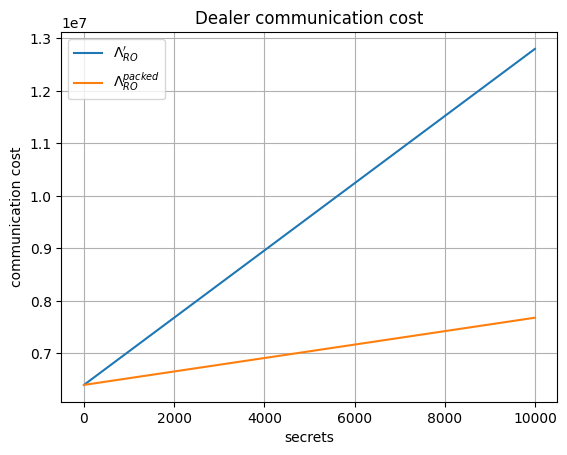
\includegraphics[width=0.7\textwidth]{figures/3pvss_communication_cost.png}
  }
  \caption{This plot compares $\Lambda_{RO}'$ and $\Lambda_{RO}^{packed}$ in terms of communication costs. 
  The x-axis represents the possible number of secrets $\ell$ when the total number of parties 
  is fixed, while the y-axis shows the communication cost for varying $\ell$ and threshold $t$. 
  The blue line corresponds to $\Lambda_{RO}'$, and the orange line corresponds to $\Lambda_{RO}^{packed}$.}
  \label{fig:3pvss_communication_cost}
\end{figure}

In the graph, we fixed the number of parties, $n=10000$, for which we varied $\ell$ with 
$1\leq t\leq \frac{n-\ell}{2}$.

\subsection{On the computational cost}

As $\Lambda_{RO}'$ is a direct extension of $\Lambda_{RO}$ 
\cite{cryptoeprint:2025/576}, the computational 
cost grows linearly with the number of secrets. And as $\Lambda_{RO}^{packed}$ is a slightly 
different approach, we save number of exponentiations in verification by a constant factor of 
$\ell$ but it costs additional group multiplications in share, verification and optiminstic 
reconstruction phases. As group exponentiations with random exponents are usually more 
expensive than group multiplications (to put that in the perspective, computing $g^x$ for 
a random $x\in\mathbb{Z}_q$ can take $\mathcal{O}(\log{q})$ group multiplications). 
Hence, the realistic increase in cost of $\Lambda_{RO}^{packed}$ due to additional 
group multiplications can be negligible. 


\begin{figure}[t!]
  \centering
  \resizebox{\textwidth}{!}{
  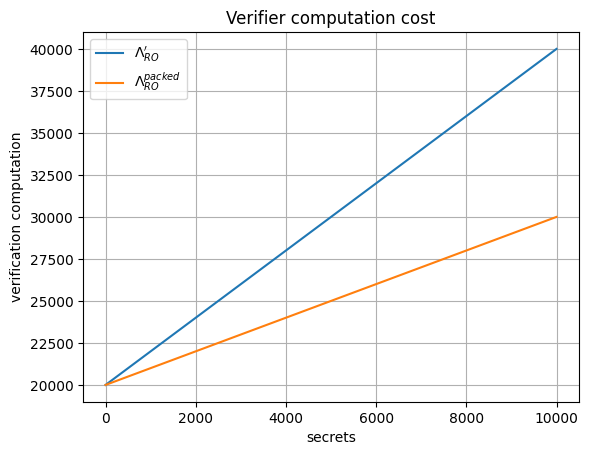
\includegraphics[width=0.7\textwidth]{figures/3pvss_verify_cost.png}
  }
  \caption{This plot compares $\Lambda_{RO}'$ and $\Lambda_{RO}^{packed}$ in terms of computation cost  
  a verifier has to bear in the verification phase. 
  The x-axis represents the possible number of secrets $\ell$ when the total number of parties 
  is fixed, while the y-axis shows the verification cost for varying $\ell$ and threshold $t$. 
  The blue line corresponds to $\Lambda_{RO}'$, and the orange line corresponds to $\Lambda_{RO}^{packed}$.}
  \label{fig:3pvss_verify_cost}
\end{figure}

Similar to the graph in previous subsection, we plotted the speculated computational costs of both the 
schemes in figure \ref{fig:3pvss_verify_cost} where we fixed the number of parties, $n=10000$, 
for which we varied $\ell$ with $1\leq t\leq \frac{n-\ell}{2}$. For this plot, we 
considered the group to be an elliptic curve over a 256-bit prime field which is 
cyclic of order a 256-bit prime $q$, i.e., each element $(x,y)$ on the elliptic curve 
is typically of 512-bit size.\par



% \section{A compact PVSS scheme}
% The relation $\pi_{PDL}^{mod-v1}$ has more potential that a new PVSS can be constructed on top of it. We 
% present it in the figure \ref{fig:compact-PVSS-ro}. 

% \begin{figure}[ht]
    \centering
    \resizebox{\textwidth}{!}{ % Further reduced the scaling factor to fit the content
    \begin{tcolorbox}[title=$\Pi_{S}^{compact}$, width=1.2\textwidth, colframe=blue!75!black, colback=blue!10, sharp corners]
        
        \textbf{Initialization:}
            All parties $\{P_i\}_{i=1}^n$ and dealer $D$ agree on the prime field $\mathbb{Z}_q$, a group 
            $(\mathbb{G},\times)$ of order $q$ with a generator $g$, random oracle $\mathcal{H}$. Also, each party 
            $P_i$ registers their public key $PK_i$ in the public ledger, where $PK_i=g^{SK_i}$ with 
            $SK_i$ being their corresponding secret key.

        \vspace{0.5em}
        \textbf{Share:}
        \begin{itemize}
            \item Dealer $D$ samples a $t$-degree polynomial $f\in\mathbb{Z}_q[X]$ uniformly at random and 
              sets $g^{f_0}$ as secret where $f_0=f(0)$.
            \item For each $1\leq i\leq n$, $D$ encrypts $f(i)=f_i$ with $PK_i$ to obtain 
              $y_i=PK_i^{f_i}$.
            \item $D$ uses $\pi_{PDL}^{AOK}$ \ref{subsec:v1} to generate AoK $\pi_{share}^{AoK}$ to prove that the 
              encryptions are valid, which is done as follows:
            \begin{itemize}
                \item Samples a $t-$degree polynomial $r\in\mathbb{Z}_q[X]$ uniformly at random and 
                computes a single commitment $c=(\prod_{i=1}^{n}PK_i^{r(i)})$.
                \item Using $\mathcal{H}$, $d=\mathcal{H}(y_1,\dots,y_n,c)$ is computed.
                \item Sets $z(X)=r(X)+df(X)$, hence $\pi_{share}^{AoK}=(d,z(X))$ is obtained. 
            \end{itemize}
            \item $D$ broadcasts the encryptions of the shares along with $\pi_{share}^{AoK}$ which 
              proves the validity of the encrypted shares, i.e., broadcasts 
              $\{y_i\}_{i=1}^n$ and $(d,z(X))$.
        \end{itemize}
        
        \vspace{0.5em}
        \textbf{Verification:}
            Given public keys $\{PK_i\}_{i=1}^n$, any entity can check 
            $\pi_{share}^{AoK}$ to verify the correctness of encrypted shares $y_1,\dots,y_n$. 
            They will output \textbf{true} or \textbf{false} based on the verification of the proof. The 
            procedure is outlined as follows:
        \begin{itemize}
            \item The entity checks if $z(X)$ is a $t-$degree polynomial or not.
            \item Checks if $d=\mathcal{H}(y_1,\dots,y_n,\frac{\prod_{i=1}^{n}PK_i^{z(i)}}{[\prod_{i=1}^n y_i]^d})$.
            \item Outputs \textbf{true} if both of the above checks are satisfied, otherwise \textbf{false}.
        \end{itemize}

        \vspace{0.5em}
        \textbf{Reconstruction:}
            Any set $\mathcal{Q}$ consisting $t+1$ honest shareholders will do the following:
            \begin{itemize}
                \item Each party $P_i\in\mathcal{Q}$ decrypts their share $y_i$ using their private key $SK_i$ 
                    corresponding to $PK_i$ to obtain $g^{f_i}$ and then they publish $g^{f_i}$ 
                    along with a DLEQ proof \ref{subsec:chaum-pedersen}, $\pi_{DLEQ}$ which proves that 
                    $g^{f_i}$ is the correct decryption of $y_i$.
                \item They can use the 
                lagrange interpolation to compute the secrets $g^{f_0}$ as follows:
                \begin{align*}
                    g^{f_0} &= \prod_{i\in\mathcal{Q}}(g^{f_i})^{\prod_{k\in\mathcal{Q},k\neq i}\frac{-k}{i}}= g^{\sum_{i\in\mathcal{Q}}f_i\prod_{k\in\mathcal{Q},k\neq i}\frac{-k}{i}}.\\
                \end{align*}
            \end{itemize}
    \end{tcolorbox}
    }
    \caption[PVSS]{$\Pi_{S}^{compact}$, a compact version of $\Pi_{S}$}
    \label{fig:compact-PVSS-ro}
\end{figure}


% \begin{theorem}
%   $\Pi_{S}^{compact}$ is secure.
% \end{theorem}

\section{Conclusion}
In this chapter, we generalized PPVSS to Packed PPVSS and presented two practical schemes based on 
Packed Shamir secret sharing. The reason to introduce the 3PVSS $\Lambda_{RO}'$ is because of its 
potential applications in some e-voting protocols. In this thesis, we wanted to mainly focused on randomness beacon 
protocols based on PVSS, due to this reason we introduced our second 3PVSS $\Lambda_{RO}^{packed}$ which is based on the
NIZK AoK $\pi_{mod-PDL}^{AoK}$ for the modified-PDL problem.\par

In the next chapter, we will revisit the randomness beacon ALBATROSS \cite{cryptoeprint:2020/644} based on PVSS, 
and replace the Packed Shamir secret sharing based PVSS with our 3PVSS $\Lambda_{RO}^{packed}$. 

%%% Local Variables: 
%%% mode: latex
%%% TeX-master: "thesis"
%%% End: 
